\part{Un corpus déjà structuré}

\clearpage
\thispagestyle{empty}
\cleardoublepage
\vspace*{\stretch{0.3}}
Le corpus sur lequel nous avons travaillé est un ensemble de fichiers XML-TEI. Ces derniers résultent d'une version numérisée des \odm{} réalisée et hébergée par le site \ia, elle-même issue du traitement des volumes physiques de l'Université de Toronto. Dans cette première partie, nous allons décrire ces différents états des \odm{} et commenter les opérations qui ont mené à leur structuration, tout en interrogeant les raisons ayant conduit le programme \timeus{} à les privilégier par rapport à d'autres versions similaires.
\vspace*{\stretch{1.7}}

\chapter{Un corpus d'imprimés}

\section{Une longue publication}
\label{part:I1_longue_pub}

La publication des trois séries des \odm{} s'échelonne sur soixante-treize années (1857-1930). Elle n'est véritablement continue que sur trois périodes, de 1857 à 1862, puis de 1885 à 1913 et enfin de 1928 à 1930. L'interruption entre 1913 et 1928 est une conséquence de la première Guerre mondiale et des difficultés budgétaires auxquelles la \sess{} doit faire face après celle-ci. La première interruption, entre 1862 et 1885, est présentée \textit{a posteriori} comme un recalibrage des objectifs de la \sess, qui considère que \og continuer à recueillir des faits sans essayer d'en faire sortir aucune conclusion (...) c'eût été (...) une preuve d'impuissance et de stérilité \fg{}\footcite[p. I]{averts1t5}. Elle se concentre dès lors sur la parution de son \textit{Bulletin} jusqu'au début des années 1880, où \og le besoin de conclusions pratiques était amplement satisfait \fg{} et \og  l'œuvre des monographies de familles \fg{} redevenait possible\footcite[p. II]{averts1t5}.

Une tentative de reprise avait déjà été effectuée en 1875 où \og un premier fascicule composé de trois monographies \fg{} avait paru\footcite[p. III]{averts1t5}. Deux autres paraissent en 1883 et 1884, et les trois sont finalement rassemblés en 1885 dans le cinquième volume de la première série\footcite[p. III]{averts1t5}. Ce volume apparaît ainsi à bien des égards comme un moment charnière dans l'histoire de la publication des \odm. En effet, les monographies suivantes des deuxième (1887-1899) et troisième série (1904-1930) sont publiées sous forme de fascicules trimestriels qui sont ensuite reliés en volumes, là où les quatre premiers tomes étaient directement parus en volumes\footnote{\cite[p. 124]{lorry}.}. Des éléments de paratexte sont systématiquement fournis aux relieurs, notamment une page de titre, une introduction au volume, un index, des \textit{errata} et une table des matières\footnote{Nous utilisons le terme \textit{paratexte} par commodité, tout en étant au fait des problèmes qu'il pose. Il suppose notamment une unité de ces textes, ce qui n'est pas le cas : cohabitent ainsi le paratexte propre aux fascicules et celui propre aux volumes finaux.}.

Le passage des volumes reliés aux fascicules trimestriels est acté par l'éditeur dans l'\textit{Avertissement} liminaire du premier fascicule de la deuxième série :

\begin{quote}
    \og La nouvelle série des \odm{} s'ouvre avec 
le présent fascicule. Le grand nombre des travaux soumis à la 
Société d'Économie sociale assure l'avenir et la régularité 
de la publication. \textit{Les monographies paraîtront désormais en 
fascicules trimestriels}\footnote{\cite[\og Avertissement \fg{}]{mono047a}. Nous soulignons.}. \fg{}
\end{quote}

Dans l'\textit{Avertissement} général de ce volume, édité en 1887 et placé immédiatement après la page de titre et le sommaire, le changement est à nouveau annoncé, mais également justifié :

\begin{quote}
    \og Quand la Société d'Économie sociale, en 1882, perdit celui qui 
avait réglé son rôle auprès de lui et après lui\footnote{Frédéric Le Play est mort le 5 avril 1882.}, elle trouva le cinquième tome des \odm{} arrêté au premier tiers de sa publication : elle acheva de le mettre au jour. Puis, voulant laisser bien distincts des travaux accomplis sous l'\oe{}il du maître, ceux dont il lui fallait dès lors prendre seule la responsabilité, \textit{elle commença en juillet 1885, sous le même titre, une nouvelle série de monographies de familles paraissant par fascicules trimestriels}\footnote{\cite[spec. p. II]{s2avert}. Nous soulignons.}. \fg{}
\end{quote}

\begin{figure}[t]
    \centering
    \begin{subfigure}[t]{0.4\textwidth}
     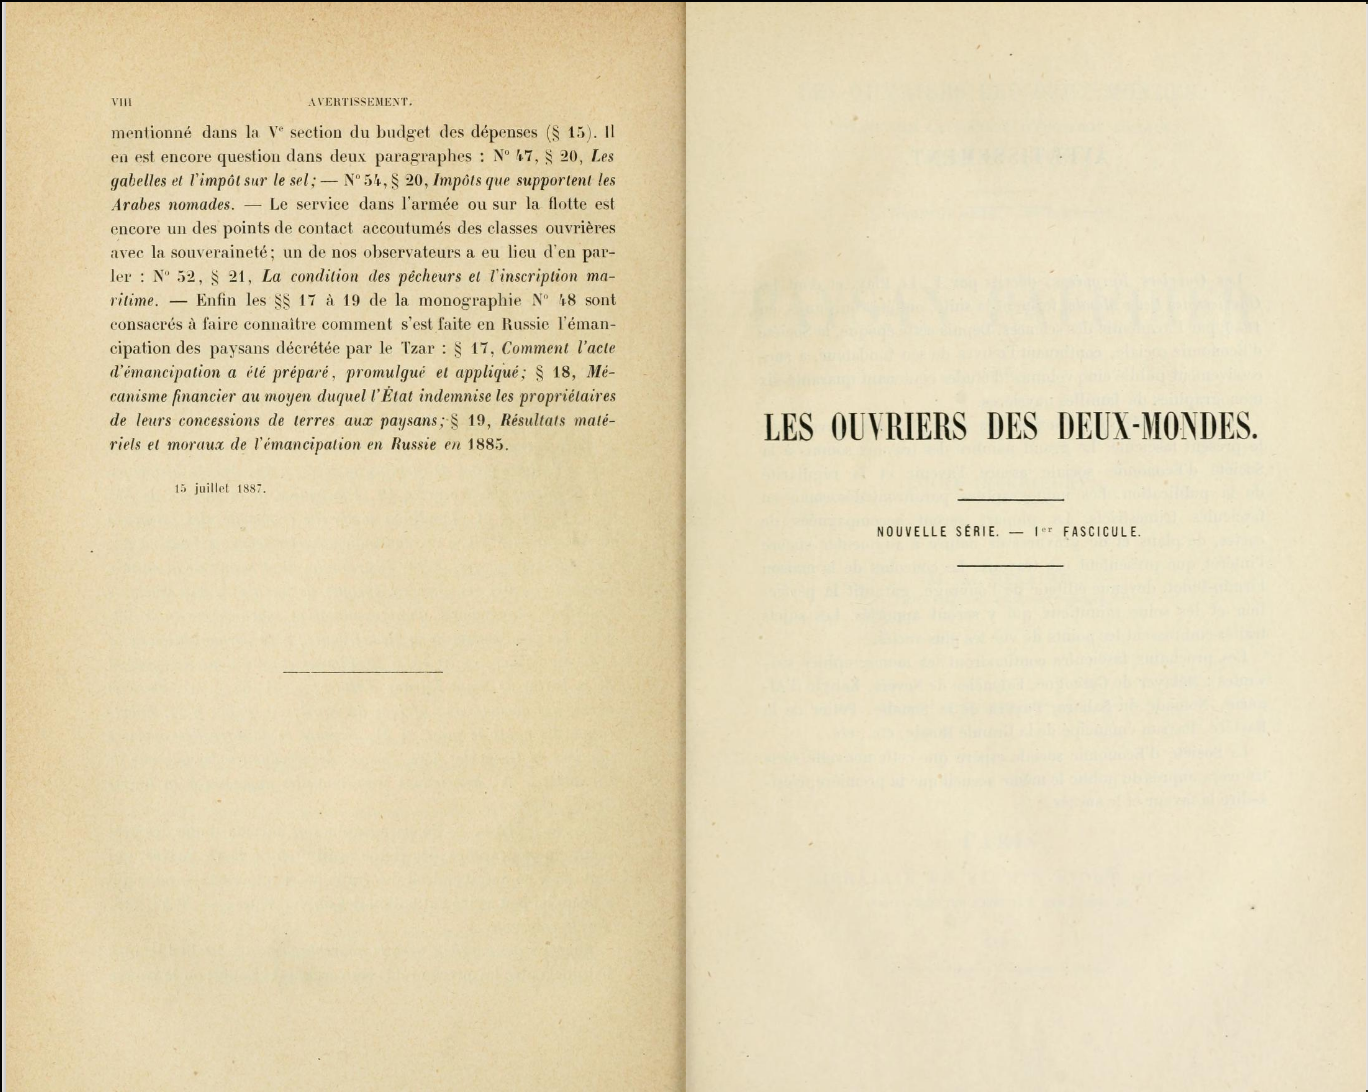
\includegraphics[width=1\linewidth]{img/odm47_ia_1.png}
     \caption{}
     \label{odm47ia1}
    \end{subfigure}
    \hspace{5pt}
    \begin{subfigure}[t]{0.4\textwidth}
     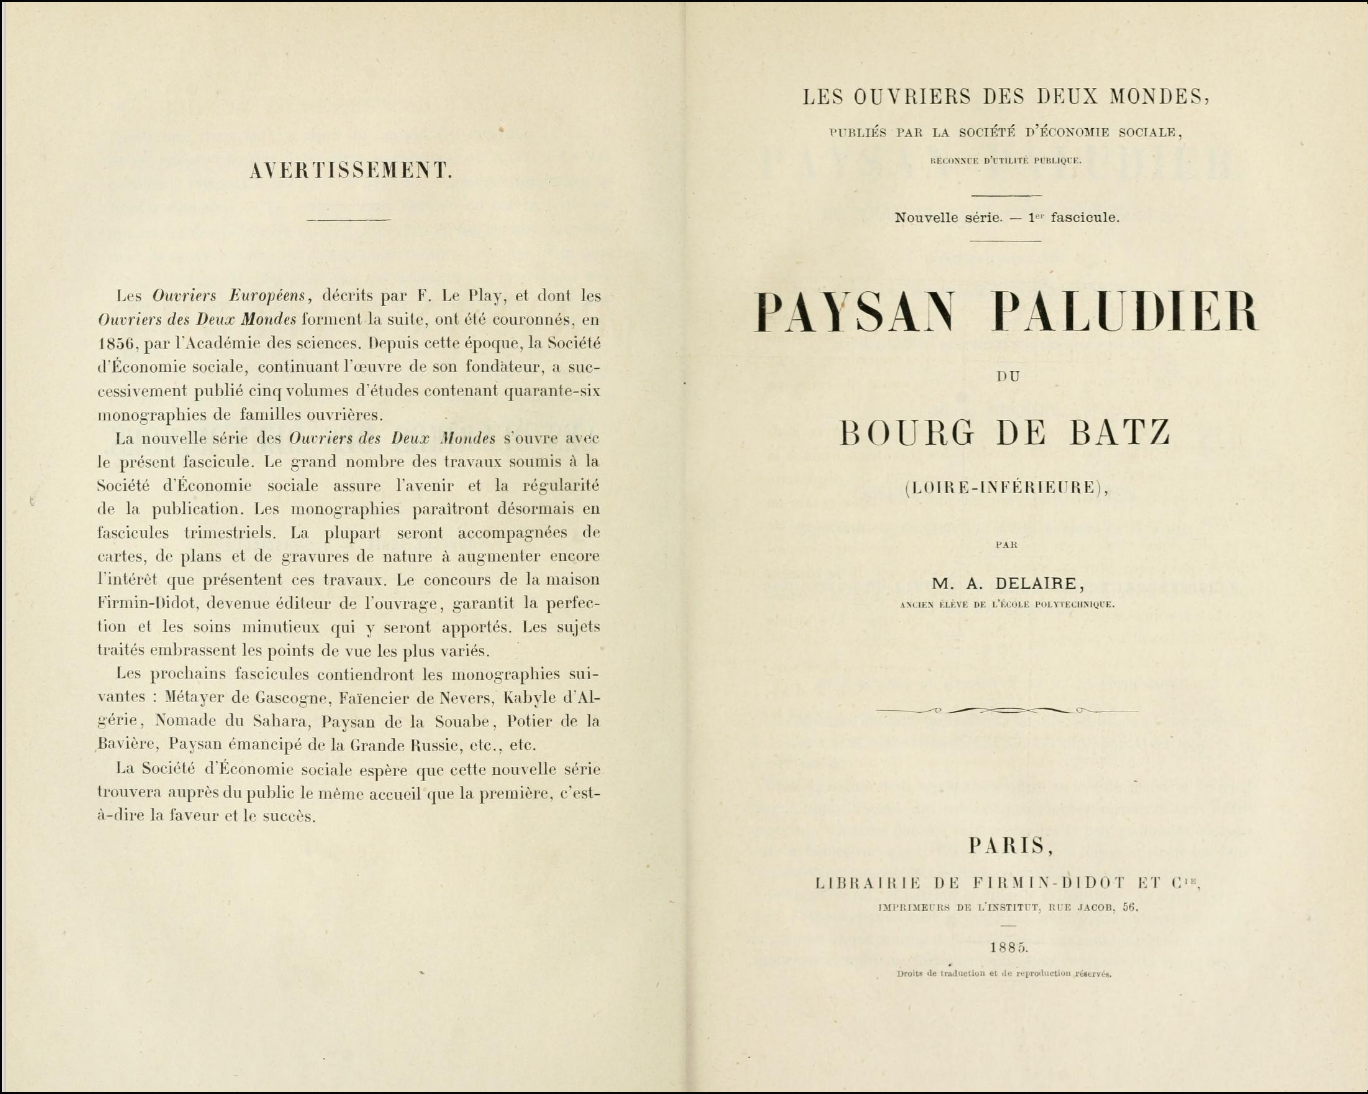
\includegraphics[width=1\linewidth]{img/odm47_ia_2.png}
     \caption{}
     \label{odm47ia2}
    \end{subfigure}
    \hspace{5pt}
    
    
    
    \begin{subfigure}[t]{0.4\textwidth}
     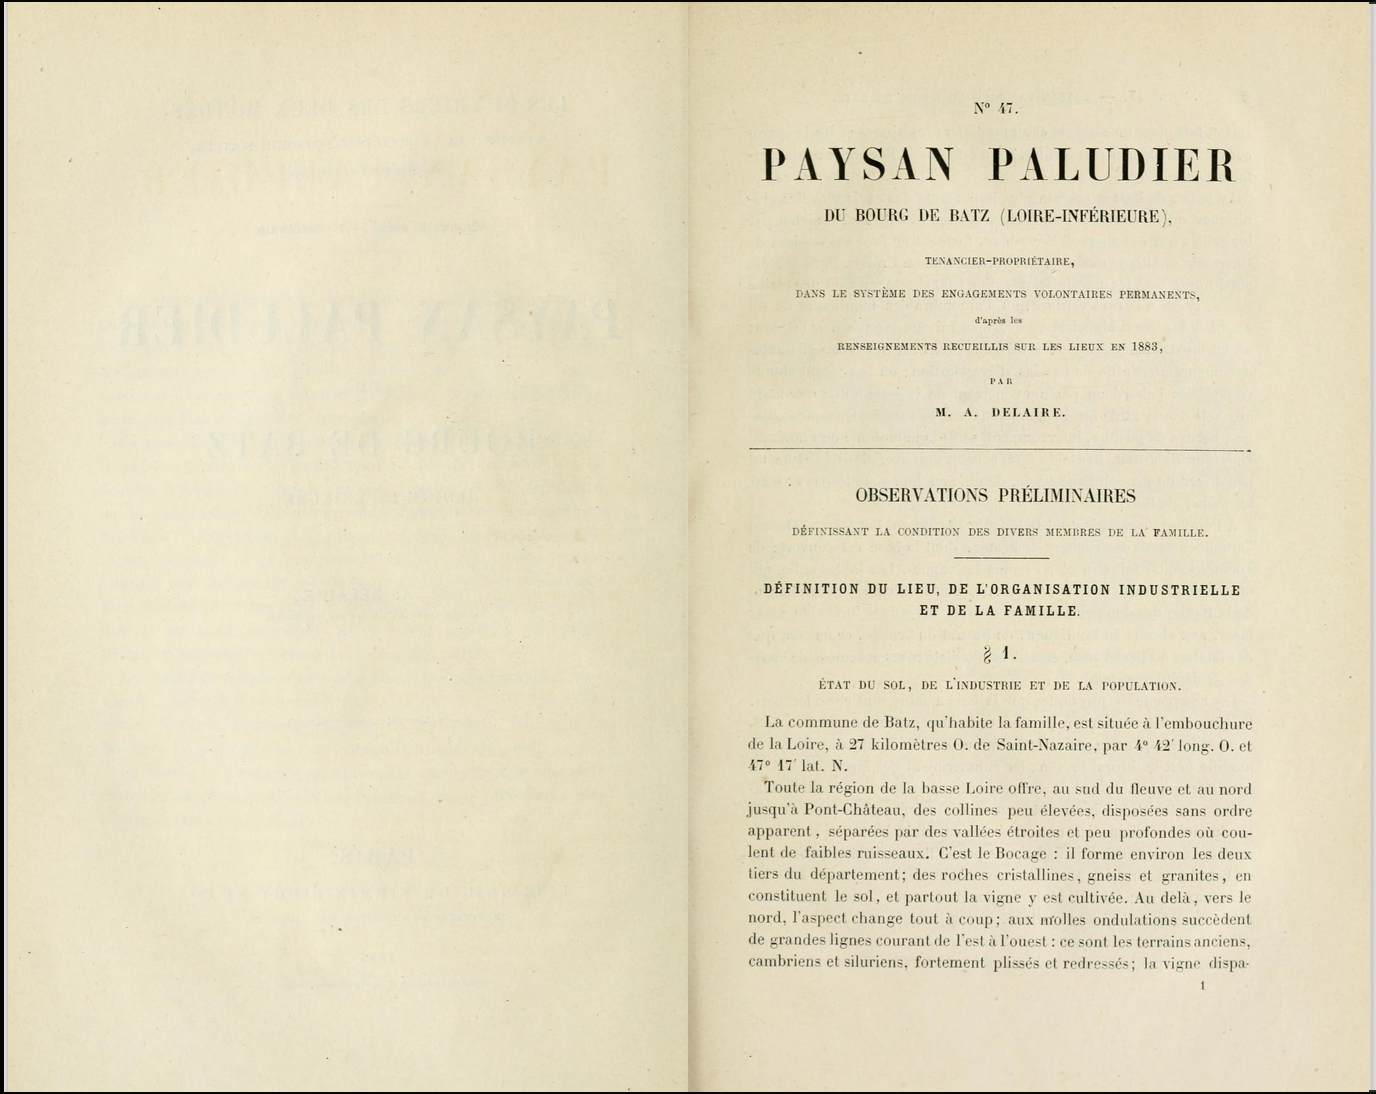
\includegraphics[width=1\linewidth]{img/odm47_ia_3.png}
     \caption{}
     \label{odm47ia3}
    \end{subfigure}
    \hspace{5pt}
    \begin{subfigure}[t]{0.4\textwidth}
     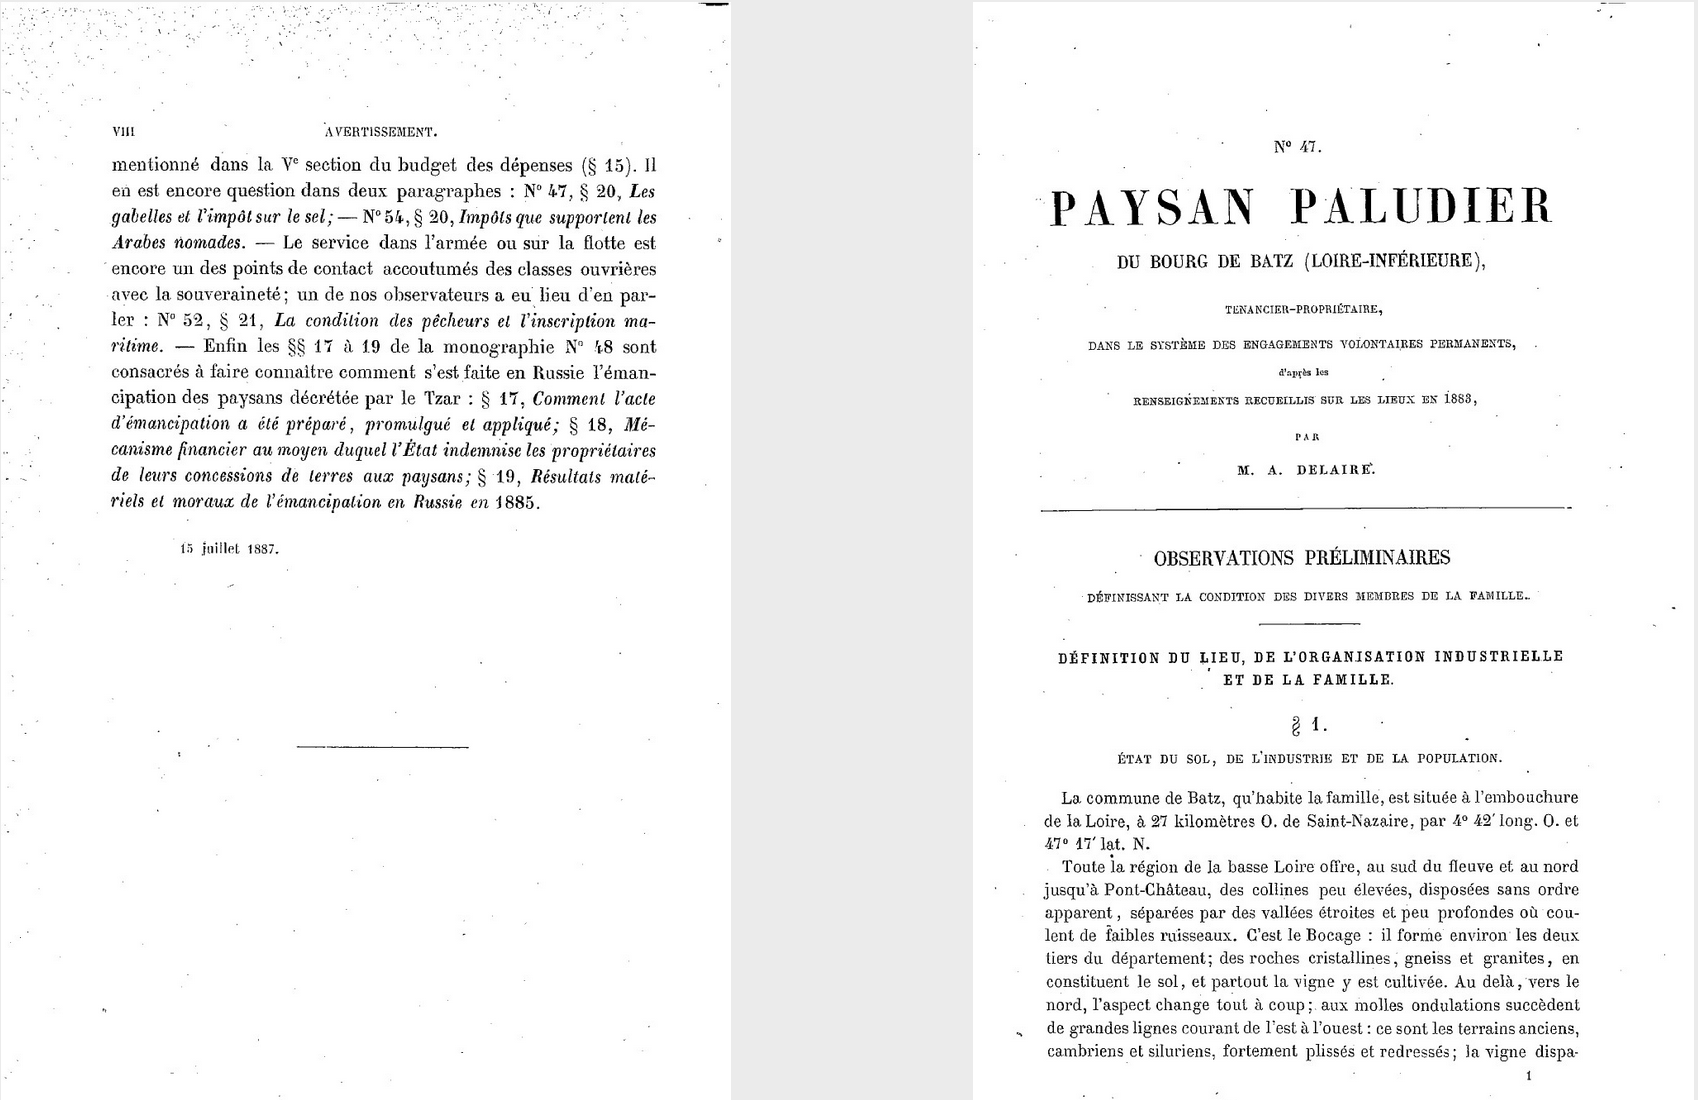
\includegraphics[width=1\linewidth]{img/odm47_bnf_1.png}
     \caption{}
     \label{odm47bnf}
    \end{subfigure}
    \caption[Comparaison des exemplaires de Toronto et de Paris]{Comparaison des exemplaires de Toronto et de Paris. (a)~Toronto. Fin de l'\textit{Avertissement} général du volume et début du fascicule. (b)~Toronto. \textit{Avertissement} du fascicule et page de titre de la monographie. (c)~Toronto. Début de la monographie. (d)~Paris. Fin de l'\textit{Avertissement} général du volume et début de la monographie.}
    \label{odm47}
\end{figure}

Deux versions de ce même volume sont à notre disposition. L'une résulte de la numérisation de l'exemplaire déposé à la Bibliothèque nationale de France à Paris et conservé par le département Philosophie, histoire, sciences de l'homme\footnote{Consultable sur \textit{Gallica} : \url{https://gallica.bnf.fr/ark:/12148/bpt6k54465138} (consulté le \today).}, la seconde se trouve à l'Université de Toronto et a été numérisée par \ia\footnote{Consultable à cette adresse : \url{https://archive.org/details/s2lesouvriersdes01sociuoft} (consulté le \today).}.

Des différences de composition existent et concernent notamment l'emplacement des page liminaires des fascicules. Ainsi, dans l'exemplaire de Toronto (\fig{} \ref{odm47ia1}, \ref{odm47ia2}, \ref{odm47ia3}), les premières pages ont été laissées à leur emplacement : la première porte au recto le titre des \odm{} et au verso l'\textit{Avertissement} que nous avons cité, la seconde est la page de titre du fascicule avec un verso vierge. Dans l'exemplaire de la Bibliothèque nationale, la première page de la monographie \no{} 47 suit la fin de l'\textit{Avertissement} général du volume : deux feuillets sont donc manquant. Ils ont été éliminés lors du processus de reliure. Les mêmes manques s'observent dans les volumes qui suivent ; on peut cependant observer que les pages propres aux fascicules ont été placées en fin de volume, après la table des matières. Il n'y a donc pas eu d'élimination systématique.

Un autre élément symptomatique de ces différences de composition se remarque dans le corpus de Toronto. La monographie \no{} 56 est la première du deuxième volume de la deuxième série\footcite{mono056a}, or elle se trouve également à la fin du volume précédent. La table des matières de ce dernier n'y fait pourtant pas référence. Ce doublon trouve sans doute son origine dans l'existence d'un fascicule surnuméraire que le relieur a choisi de conserver, quitte à l'implanter au mauvais endroit.

Ces exemples illustrent le fait que laisser aux acheteurs le soin de relier les fascicules pour composer le volume final revient à éloigner ce dernier de l'\oe{}uvre originelle, chaque nouvelle opération de reliure donnant naissance à un nouveau document. Les relieurs ont en effet pu choisir de conserver ou de ne pas conserver les pages propres aux fascicules, à l'instar des feuillets de l'exemplaire de Toronto. Il n'existe donc pas un modèle ayant autorité dans la composition des \odm{} --- en dépit du fait que les volumes de la Bibliothèque nationale de France, issus du dépôt légal, ont dû être versés par l'éditeur, \cad{} la Société internationale des études pratiques d'économie sociale.

Pour le projet \timeus{}, cela signifie que le corpus retenu pour le traitement informatisé et la publication finale ne peut être qu'une version de l'\oe{}uvre que représente les \odm.

\section{La structure logique des monographies}

Un élément remarquable traverse la centaine de monographies des \odm{} : une même structure logique que les éditeurs ont tenté de maintenir tout au long de la publication.

Cette structure est l'incarnation de la méthodologie leplaysienne des monographies de familles. Le terme \textit{monographie}, \og emprunté à l'histoire naturelle et à la médecine \fg{}, qualifie au \textsc{xix}\ieme ~siècle une \og étude scientifique, minutieuse et détaillée, portant sur un objet ou un phénomène circonscrit \fg{}\footnote{\cite[p. 12]{savoye2}.}. La démarche monographique cherche à embrasser à travers l'observation directe des phénomènes inatteignables pour la démarche statistique, à laquelle elle s'oppose\footnote{Voir en particulier la charge de F. Le Play contre les statisticiens dans son introduction aux \textit{Ouvriers européens} de 1855 : \og La méthode des statisticiens n'est pas l'observation directe des faits ; c'est la compilation et l'interprétation plus ou moins plausible de faits recueillis à des points de vue fort différents, étrangers pour la plupart à l'intérêt scientifique. Malgré leur généralité apparente et leur séduisante régularité, les statistiques ont médiocrement contribué au progrès de la science sociale \fg{} : \cite[p.~11]{oe1855}.}.

Avant les \odm, Frédéric Le Play s'attelle aux \textit{Ouvriers européens}, recueil paru en 1855 et réédité de 1877 à 1879. Cette série contient trente-six (1\iere{}~éd.) puis cinquante-sept (2\ieme{}~éd.) monographies issues d'enquêtes menées entre 1833 et 1853\footnote{Inventaire complet dans \cite[p. 106-112]{lorry}.}. Les \odm{} se présentent comme une suite élargie à des espaces extra-européens de ce premier mouvement, dont ils reprennent la démarche, la structure et auquel ils font régulièrement référence par un système de renvoi. La structure logique des \odm{}, dont le premier volume est publié en 1855, est donc déjà présente dans \textit{Les Ouvriers européens}.

Elle procède d'une méthode d'observation sur laquelle Le Play revient en 1862, au moment de la parution du quatrième volume des \odm{}. Le titre de cette méthodologie précise néanmoins qu'elle a déjà fait ses preuves pour les \textit{Ouvriers européens} : \textit{Instruction sur la méthode d'observation dite des monographies de familles, propre à l'ouvrage intitulé} Les ouvriers européens\footcite{instruction62}.

L'\textit{Instruction} est divisée en quatre parties suivies d'une cinquième faisant office de conclusion. Dans la première, Le Play circonscrit son champ d'observation à la famille ouvrière\footcite[I., \og Remarques préliminaires sur l'étude des faits sociaux et sur la méthode des monographies de familles \fg{}, p. 15-16]{instruction62}, érigée en \og clef de compréhension des organisations sociales \fg{}\footcite[p. 15]{savoye2}. La phase d'observation est ensuite divisée en étapes \footcite[II., \og Règles à suivre pour procéder à l'observation des faits sociaux \fg{}, p. 17-19]{instruction62}, savoir l'observation des faits, l'interrogatoire de l'ouvrier et celui des personnes tiers\footcite[p. 16]{savoye2}.

La troisième partie est celle où Le Play expose la structure logique qu'il utilise à partir de 1855 et que ses \og continuateurs \fg{}\footnote{Nous désignons par ce terme le groupe d'individus qui a participé à l'entreprise des \odm{} après la mort de Le Play, sans entrer dans les débats sur l'existence ou non d'une \og école leplaysienne \fg{}. De fait, un schisme a lieu à la fin des années 1880 : \cite{savoyecontinuateurs}.} reprennent jusqu'en 1930. Elle est construite en miroir aux différentes phases de l'observation sur le terrain : à l'observation des faits répond la section des\textit{ Observations préliminaires}, à l'interrogatoire de l'ouvrier celle des \textit{Budgets} et aux contacts avec les tiers celle des \textit{Notes}\footcite[III., \og Précis des faits à observer --- Établissement des budgets \fg{}, p. 20-31]{instruction62}.

Le miroir est cependant légèrement déformant, afin de satisfaire au \og hiatus \fg{} propre à la démarche leplaysienne, qui différencie les \og faits observés \fg{} des \og faits décrits \fg\footcite[p. 87]{baciocchi2}. L'observation est en effet \og contrainte par l'évidence des choses \fg{} là où la description, \og parce qu'elle suppose de désigner précisément ce qu'on évoque, repose sur un calibrage sémantique \fg{}\footcite[p. 87-88]{baciocchi2}. Les monographies se trouvent du côté de la description des faits, leur structure logique n'est donc pas qu'un simple plan de rédaction, elle procède d'une démarche intellectuelle réglée par Le Play qui doit être appliquée pour garantir la validité de la démonstration.

Cette structure (\ann{} \ref{structure}) possède trois niveaux de titre : les parties~(A, B, C), les sections~(I, II, etc.) et les paragraphes~(§1, §2, etc.). La partie~C (\textit{Notes}) n'a pas recours au deuxième niveau et ne contient que des paragraphes.

\begin{figure}[h]
    \centering
    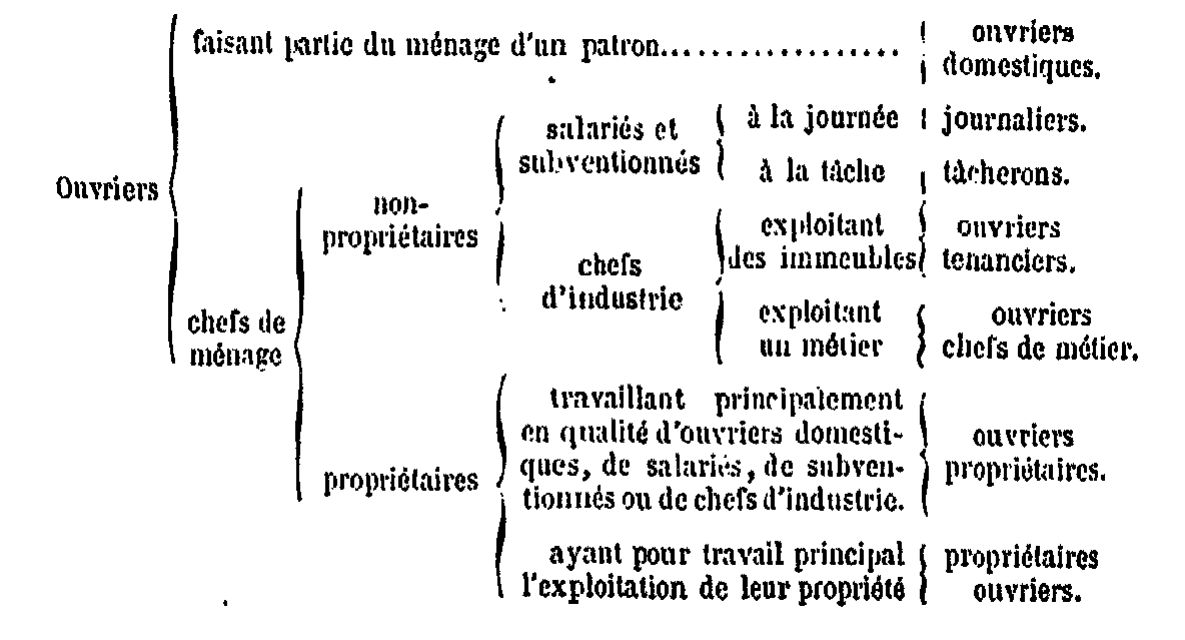
\includegraphics{img/tabl_titres.jpg}
    \caption[Tableau des sept situations principales que les ouvriers peuvent occuper successivement]{\og Tableau des sept situations principales que les ouvriers peuvent occuper successivement dans les quatre systèmes sociaux pour s'élever des rangs inférieurs de la hiérarchie industrielle à la condition de propriétaires ou de chefs d'industrie. \fg{}, permettant de construire le titre d'une monographie de famille (capture d'écran de \textit{Gallica}).}
    \label{tabletitre}
\end{figure}

La première partie~(A) est la page de titre. Le titre de la monographie est présenté comme le \og résumé \fg{} de celle-ci, et doit pour cela contenir quatre éléments imprescriptibles : \og 1° la profession de l'ouvrier, 2° la population dont il fait partie, 3° la nature des engagements qu'il contracte pour se procurer des moyens de travail, 4° la situation qu'il occupe dans l'organisation sociale caractérisée par cet engagement \fg{}\footcite[p. 20]{instruction62}. Ainsi, en dépit du fait que Le Play ne considère pas explicitement la page de titre comme une composante de sa structure, l'importance qu'il donne au titre en lui-même a conduit le projet \timeus{} à l'interpréter comme telle. Un tableau pour construire ce titre est d'ailleurs mis à la disposition des monographes (\fig{} \ref{tabletitre}\footcite[p. 21 .]{instruction62}).

\section[Continuité et discontinuité]{Continuité et discontinuité dans la structure logique}

En dépit de son aspect monolithique, la structure logique des monographies de familles subit plusieurs ajustements au cours de la publication. Certains, uniquement de circonstance, sont des évènements mineurs, là où d'autres sont des changements significatifs adoptés pour la suite de la publication.

La monographie \no{} 85 représente ainsi un tournant dans la numérotation des titres de paragraphe, sans pour autant changer leurs libellés (\ann{} \ref{structure}). En effet, la numérotation cardinale est étendue au dernier paragraphe des budgets (\textit{Comptes annexés aux budgets}) et remplace la numérotation alphabétique utilisée auparavant dans la partie \textit{Notes}.

Pourquoi cette uniformisation intervient-elle à partir de cette monographie, en plein milieu du cinquième volume ? Nous avons vu plus haut qu'il représentait un tournant dans la publication des \odm, notamment en raison de la mort de Frédéric Le Play qui intervient avant qu'il ne soit achevé. Il est possible que le départ du fondateur de la série ait permis d'opérer des changements dans la structure qu'il avait créée, ou bien que ce soit Le Play lui-même qui ait souhaité ces changements. Quoi qu'il en soit, il y a une volonté claire de renforcer la solidité de la démonstration en rassemblant ces différents paragraphes en un seul bloc par le biais d'une numérotation cardinale continue. Le nombre moyen de paragraphes est de vingt-et-un ; la monographie la plus longue, composée de trente-cinq paragraphes, étant la \no{} 64, intitulée \textit{Paysans corses en communauté, porchers-bergers des montagnes de Bastelica}\footcite{mono064a}.

Ce même volume est l'occasion pour la \sess{} d'agréger aux \odm{} un type de monographie déjà introduite dans la ré-édition des \textit{Ouvriers européens} (1877-1879), le précis\footcite[p. 102]{lorry}. Elle le définit comme un document qui, \og n'ayant pas la forme complète des travaux auxquels ce recueil est destiné [les monographies de familles], offre néanmoins assez d'intérêt pour avoir été annexé à la description d'une famille de même nationalité \fg{}\footcite[p. II]{averts2t1}. Il s'agit d'un texte court, d'une quinzaine de pages environ, qui, tout en ayant le même propos qu'une monographie, est fortement \og allégé \fg{}\footcite[p. 7]{chenu}.

Cet allègement se remarque à travers deux traits caractéristiques. Le premier est la suppression du paragraphe 16 et la réduction des paragraphes 14 et 15 consacrés aux budgets. Ils sont en effet réduits à quelques lignes, là où il s'agit de tableaux de plusieurs pages dans les  monographies de familles. Le précis \no{} 92 \textit{bis} est le seul à posséder un paragraphe 16, mais les 14 et 15 sont rassemblés en une seule section\footcite[p. 78-81]{mono092b}. Le second trait caractéristique consiste en des notes extrêmement courtes (un à trois paragraphes, à l'exception du précis \no{} 66 \textit{ter} qui en compte six\footcite[p. 158-172]{mono066c}).

Les libellés des titres peuvent également être modifiés. Celui de la deuxième partie (\textit{Observations préliminaires}) est absent des précis \no{}~58 \textit{bis}\footcite[p. 153]{mono058b} et 66~\textit{bis}\footcite[p. 125]{mono066b}. Ceux des paragraphes sont également placés en italique au début du texte dans quatre précis (\no{} 58~\textit{bis}, 66~\textit{bis}, 85~\textit{bis}\footcite{mono085b}, 90~\textit{bis}\footcite{mono090b}).

Les trois premiers précis sont des cas particuliers, puisqu'à l'inverse des suivants ils ne sont pas formellement détachés de la monographie dont ils découlent (\no{}~41\footcite[p. 188-196]{mono041a}, 42\footcite[246-258]{mono042a} et 43\footcite[p. 300-305]{mono043a}) mais sont traités comme une section de la partie \textit{Notes}. Il n'y a ni grandes parties ni titres de paragraphe, seul le niveau intermédiaire ayant été retenu : les sections I à IV dans les trois, et un court budget dans les deux derniers.

Un dernier facteur de discontinuité au sein des \odm{} et de sa structure logique doit être signalé : il s'agit des deux monographies d'ateliers que l'on trouve dans la troisième série. La première s'intéresse à la société générale des papeteries du Limousin (1904\footcite{mono472a}) et la seconde à  une usine hydraulique d’éclairage et de transport de force sur la Loire (1908\footcite{mono473a}). La monographie d'atelier est théorisée par Émile Cheysson, une des grandes figures de la \sess après la mort de Le Play\footcite[p. 336-337]{savoyecontinuateurs}, pour qui le \og foyer cesse d'être le centre unique de notre activité et cède à l'atelier une partie de ses attributions primitives \fg{}\footnote{Émile Cheysson, \og La monographie d'atelier et les Sociétés d'économie sociale \fg{}, \textit{La Réforme sociale}, 15 mai 1887, p. 545 --- cité dans \cite[p. 23]{savoye2}.}.

Il s'agit d'une rupture importante avec l'objectif initial des \odm, mais également d'un signe de la volonté de la collection de s'adapter à son temps. Ces deux textes ne peuvent néanmoins pas reprendre la structure logique initiale, uniquement applicable aux familles. Néanmoins, on trouve dans leur organisation des traits similaires : trois parties (\textit{Organisation commerciale de l'atelier}, \textit{Organisation du travail} et des \textit{Appendices} faisant fonction de notes), un second niveau signalé par une numérotation en romain et des paragraphes qui peuvent être titrés ou non\footcite[p. 337]{savoyecontinuateurs}.

Ces modulations dans l'application de la structure définie par Frédéric Le Play sont importantes pour le projet \timeus. Son but étant de mettre à la disposition de la communauté scientifique les monographies des \odm{} sous la forme de fichiers XML-TEI, il est nécessaire qu'il étudie cette structure et qu'il fasse la part entre ses moments de continuité et de rupture. Ceux-ci doivent en effet être pris en compte dans l'établissement du schéma d'encodage.

\chapter{Des numérisations multiples}

Avant d'établir le schéma d'encodage des \odm, il est nécessaire de disposer d'une version digitale du corpus \og papier \fg{} pour réaliser une opération de transcription automatique. Or, comme nous l'avons déjà signalé, les \odm{} ont bénéficié des programmes de numérisation des ressources des bibliothèques.

Un corpus se trouve notamment sur le site \gb, mais il n'est important que d'un \pov{} quantitatif et non pas qualitatif. En effet, les treize volumes ne sont pas accessibles dans leur intégralité. Cet accès restreint est regrettable, dans la mesure où \gb{} n'a pas numérisé un seul corpus, mais plusieurs issus de bibliothèques italiennes, françaises et américaines (\ann{} \ref{numgb}). Disposer de tous ces exemplaires aurait permis un relevé plus fin des différences de composition. Notons que par l'intermédiaire de la \textit{HathiTrust Digital Library }, une bibliothèque numérique lancée en 2008 et agrégeant les livres numérisés par \gb, \ia{} et certaines bibliothèques universitaires, il est possible de consulter à des numérisations pour lesquelles l'accès est restreint par Google.

Le projet \timeus{} s'est donc orienté vers les deux seuls corpus complets, hébergés par la Bibliothèque nationale de France et le site \ia.

\section{Les volumes de la Bibliothèque nationale de France}

Les trois séries des \odm{} ont été mises en ligne sur le site \textit{Gallica} de la Bibliothèque nationale de France le 15 octobre 2007\footnote{Notice de la numérisation : \url{https://gallica.bnf.fr/ark:/12148/cb32830863r/} (consulté le \today).}.

Les volumes sont téléchargeables en trois formats :

\begin{itemize}
    \item PDF (\textit{Portable Document Format}), qui préserve la mise en page du document telle qu'elle a été définie par son auteur ;
    \item TXT, qui contient uniquement du texte brut, \cad{} des chaînes de caractères (ce qui n'intéresse pas le programme \timeus, qui souhaite obtenir les images des pages de chaque volume) ;
    \item JPEG (\textit{Joint Photographic Experts Group}), qui permet de compresser les images avant de les enregistrer.
\end{itemize}

Le téléchargement au format JPEG n'est possible que pour la page en cours de visualisation par l'utilisateur. Seul le téléchargement au format PDF permet d'obtenir l'ensemble des images, avec l'inconvénient qu'elles sont toutes rassemblées en un seul fichier, ce qui complique le traitement à la chaîne.

Le corpus numérisé sur \textit{Gallica} n'est ainsi pas exploitable par le programme \timeus. Cela est regrettable dans la mesure où, comme nous l'avions signalé plus haut, il s'agit des exemplaires issus du dépôt légal et donc déposés par l'éditeur des \odm. Il s'agissait de l'unique occasion d'avoir avec certitude la vision que Frédéric Le Play et la \sess{} avaient de leur travail.

\section{Les volumes d'\ia}

\ia{} est un organisme privé à but non lucratif fondé en 1996 par Brewster Kahle. Son objectif premier, tel qu'annoncé dans son \textit{manifeste}, est de \og collecter les données publiques sur Internet pour bâtir une bibliothèque digitale \fg{}\footnote{\og \textit{The Internet Archive is such a new organization that is collecting the public materials on the Internet to construct a digital library} \fg{} : \cite{Brewster1} (cité dans \cite{Brewster2}).}. Cet archivage du web est accessible grâce à l'outil \textit{Wayback Machine}, lancé en octobre 2001\footcite[p.344]{panos} mais prévu dès le lancement d'\ia\footnote{\textit{We possess the capability of supplying documents that are no longer available from the origi- nal publisher, an important function if the Web’s hypertext system is to become a medium for scholarly publishing. Such a service could also prove worthwhile for business research.} : \cite[p.83]{iamanifest}.}. À partir de 2000, l'organisation commence à archiver les programmes de télévision, les musiques et les films numériques~; en 2001, c'est au tour des livres de faire leur entrée sur ses serveurs\footcite[p. 3-4]{Brewster2}.

\ia{} commence ses digitalisations en tant que participant au projet \textit{Million Book} de l'Université Carnegie-Mellon de Pittsburgh, et se met à digitaliser par lui-même en se rendant dans les bibliothèques universitaires à partir de 2005\footcite[p. 4]{Brewster2}. La digitilasation est faite page par page au moyen de scanners\footcite[p. 4]{Brewster2}. Les livres ainsi numérisés sont accessibles  et téléchargeables librement, sans aucune restriction, ce qui constitue le principal avantage du site, à l'image de \textit{Gallica} et à l'inverse d'autres plates-formes comme \gb\footcite[p. 1]{Brewster2}. Par rapport à \textit{Gallica}, \ia{} offre beaucoup plus de formats pour le téléchargement de ses fichiers\footnote{Liste complète : \cite[p. 33]{chague}.}.

Les exemplaires des \odm{} numérisés sur \ia{} sont conservés à la \textit{John P. Robarts Research Library} de l'Université de Toronto. Leurs mises en ligne ont été réalisées en novembre 2008, mise à part le fascicule 17 \textit{bis} de la série 3, ajouté en mars 2010.

\section{Choix du corpus à numériser}

\begin{figure}[h]
    \centering
    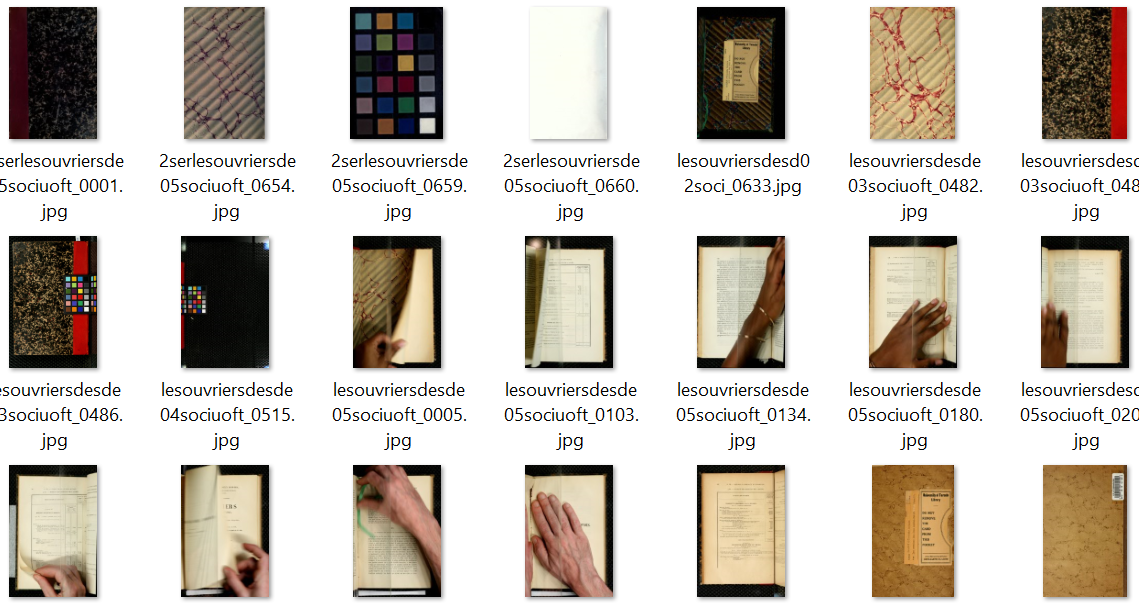
\includegraphics[width=15cm]{img/ex_tri.png}
    \caption[Images exclues du lot à transcrire]{Exemples d'images exclues du lot à transcrire (source : Alix Chagué, \url{https://timeus.hypotheses.org/626}).}
    \label{fig:ex_tri}
\end{figure}

Le téléchargement depuis \ia{} permet d'obtenir un dossier contenant le fichier image de chaque page au format JPEG (en l'occurrence JPEG 2000, abrégé en JP2) avec une qualité maximale\footcite{chague2}. C'est donc pour ce corpus et ce format qu'a opté le programme \timeus. Cela représente 7 190 fichiers images, pour un poids de 3,3 Go\footcite{chague2}.

L'ensemble a été versé sur un espace de stockage créé grâce au service \sharedocs{} de la TGIR Huma-Num. Adopté en mai 2018 à l'initiative de l'équipe ALMAnaCH, ce service est gratuit, français et sur-mesure (l'espace de stockage est alloué à la demande)\footcite[p. 33-34]{chague2}. Le \sharedocs{} permet également de centraliser l'ensemble des fichiers image du programme \timeus.

Choisir le corpus d'\ia{} n'est pas sans conséquence, notamment en raison du caractère incomplet du corpus. Les fascicules contenant les six dernières monographies (\no{}~109 à 114) et les précis qui les accompagnent (\no{}~109~\textit{bis} à 111~\textit{bis}) n'ont en effet pas été numérisés. De fait, nous ne les avons trouvés qu'à une seule adresse sur Internet : il s'agit de l'exemplaire de l'Université de Princeton numérisé par \gb{} et accessible par le truchement de la \textit{HathiTrust Digital Library} (\ann{} \ref{numgb}). Il contient les monographies \no{}~108 à 112 et constitue donc le troisième volume de la troisième série. Nous n'avons pas trouvé d'exemplaires numérisés des deux dernières monographies, publiées à la fin des années 20 du \textsc{xx}\ieme~siècle

Ce corpus comporte également divers biais liés à l'impression, dont des titres appartenant à la structure logique qui n'ont pas été imprimés (\ann{} \ref{ann:deficit-transcr}), sans que l'on puisse déterminer s'il s'agit d'une erreur de composition ou d'une suppression volontaire par les éditeurs. 

Notons qu'en dépit de ces écueils, toutes les monographies relatives au textile et qui intéressent directement le programme \timeus{} sont présentes dans le corpus d'\ia.

À l'issue du téléchargement, il a fallu procéder à un contrôle de la qualité des fichiers, afin de détecter et de retirer les images présentant des imperfections\footcite{chague2}. Ces dernières étaient principalement dues à des erreurs de cadrage ou à des vues prises alors que la main de l'opérateur ou de l'opératrice était toujours présente dans le champ de l'image (\fig{} \ref{fig:ex_tri}).

\begin{figure}[h]
    \centering
    \begin{subfigure}[t]{0.4\textwidth}
     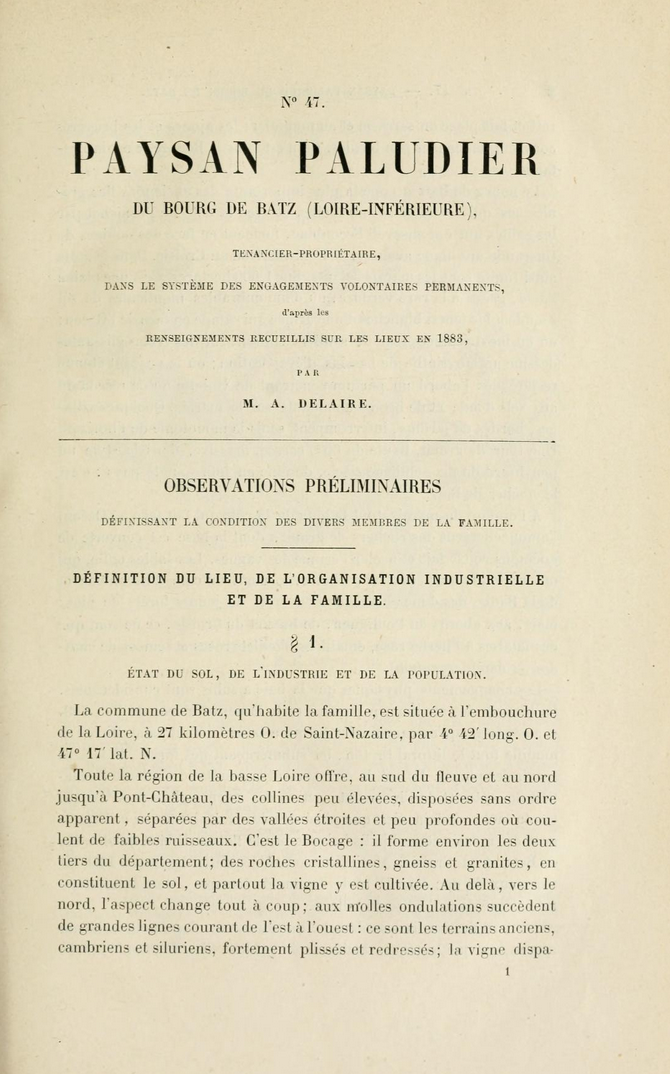
\includegraphics[width=0.7\linewidth]{img/title_s2t1_m47_p1.png}
    \end{subfigure}
    \hspace{5pt}
    \begin{subfigure}[t]{0.4\textwidth}
     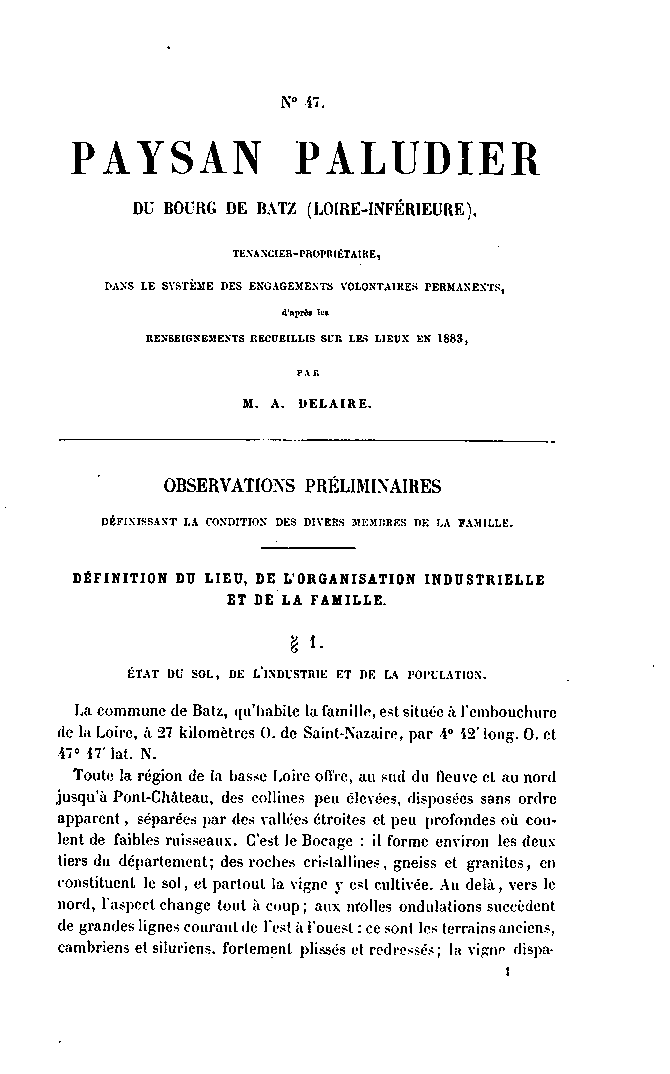
\includegraphics[width=0.7\linewidth]{img/title_binarize.png}
    \end{subfigure}
    \caption[Exemple d'une binarisation]{Exemple d'une binarisation : s. 2 vol. 1, \no{} 47, p. 1.}
    \label{fig:binarisation}
\end{figure}

Enfin, les images retenues ont été binarisées, \cad{} passées en valeur de noir ou blanc (\fig{} \ref{fig:binarisation}). Cette opération permet d'augmenter la qualité des textes et donc leur détection par les programmes de transcription automatique. Un autre avantage est qu'elle supprime les annotations manuscrites, par exemple celles ajoutées par les agents des bibliothèques et relatives au classement du volume.

Dès lors que le corpus était nettoyé, les opérations de transcription et d'encodage pouvaient débuter.

\chapter{Un encodage automatique}

\section{Choix de l'automatisation}
Le programme \timeus{} a choisi de procéder lui-même à la transcription des treize volumes des \odm{} et à l'encodage du texte brut ainsi obtenu. 

Cela n'était pas envisagé ainsi au départ, un budget ayant été prévu pour externaliser cette étape. Néanmoins, l'équipe ALMAnaCH d'Inria a fait valoir les risques inhérents à une telle opération, et notamment la difficulté à rédiger un cahier des charges suffisamment rigide pour pouvoir contrôler les différentes étapes de réalisation et les orientations scientifiques décidées lors de celles-ci.

Le choix s'est donc porté sur une réalisation en interne avec la possibilité de la conduire manuellement (un humain réalise les transcriptions avant de les encoder) ou automatiquement (un humain écrit un programme qui prend les images en entrée et fournit des fichiers XML en sortie)\footcite[p. 52]{chague}. La solution du travail manuel avait été envisagée dans un premier temps, notamment par le Centre Maurice-Halbwachs, grâce au recrutement d'un(e) ingénieur(e) d'études à temps plein pour six mois\footcite[p. 52]{chague}. 

ALMAnaCH a cependant proposé de prendre en charge l'écriture du programme permettant d'automatiser l'opération, en insistant sur les apports méthodologiques et scientifiques que cela représenteraient pour le programme\footcite[p. 52]{chague}. Le succès d'une telle opération lui permettrait en effet de développer ses compétences dans l'acquisition et l'encodage automatique de texte imprimé.

Ajoutons que cette proposition correspond à la dynamique interne dont nous avons constaté la prégnance sur les membres d'ALMAnaCH dès le début du stage. Une réflexion y est sy
stématiquement menée pour étudier l'opportunité d'automatiser les tâches répétitives dans un objectif évident de gain de temps, mais également de développement expérimental de nouvelles techniques de traitement des fichiers.

Pour mener à bien cette phase du programme, deux contrats d'ingénieur d'études de trois mois chacun (octobre à décembre 2018, février à mai 2019) ont été financés. La fiche de poste comptait sept missions\footnote{Informations transmises par Alix Chagué.} :

\begin{itemize}
    \item Réaliser un benchmark de toutes les solutions d'\ocr{} disponibles et adaptées pour le projet ;
    \item Établir une méthodologie de traitement des documents ;
    \item Télécharger les images, les contrôler et les pré-traiter ;
    \item Réaliser l'\ocr{} ;
    \item Analyser la structure logique des enquêtes pour identifier les indices textuels et typographiques permettant la structuration des transcriptions ;
    \item Établir un schéma TEI traduisant la structure logique ;
    \item Rédiger un programme cherchant ces indices et implémentant le schéma TEI.
\end{itemize}

\section{Le script \textsc{LSE-OD2M}}

La transcription automatique d'un document imprimé nécessite l'usage d'un logiciel d'\ocr{} (\textit{Optical Character Recognition}, en français \textit{reconnaissance optique de caractères}). Quatre étapes sont nécessaires afin d'obtenir un résultat satisfaisant : préparer les images en amont afin de faciliter la reconnaissance des caractères, segmenter l'image en zones d'information, extraire le texte et enfin contrôler et corriger le rendu\footcite[p. 1]{karpinski}.

Nous avons déjà évoqué la préparation des images dans le chapitre précédent, la correction correspondant quant à elle au travail produit pendant notre stage. Nous nous arrêterons donc sur les deuxième (segmentation) et troisième (transcription automatique) phases dans le propos qui suit, en y adjoignant la structuration du texte sous forme de fichiers XML-TEI.

Sur ces trois étapes, les deux dernières ont été entièrement prises en charge par un script Python dénommé \textit{Logical Structure Extraction from Les Ouvriers des Deux Mondes} (\lse), écrit par Alix Chagué de février à mai 2019.

\subsection{Segmentation}

Le but d'une segmentation est d'identifier dans l'image d'un texte des zones qui correspondent à des sous-ensembles logiques de ce texte. Il peut s'agir de paragraphes, de lignes ou de mots, la granularité pouvant être poussée jusqu'aux caractères\footcite[p. 3]{karpinski}. Ce moment est crucial pour l'\ocr, puisque la reconnaissance des caractères s'effectuera sur les zones ainsi segmentées\footcite[p. 3]{casey}. Il est identifié depuis de nombreuses années\footcite[p. 4]{casey} comme une source majeure des erreurs présentes dans le résultat final\footcite[p. 120]{elagouni}.

Plusieurs caractéristiques des \odm{} facilitent leur transcription. D'une part, il s'agit d'un imprimé du \textsc{xix}\ieme ~siècle, ce qui garantit un texte relativement régulier dont l'alphabet correspond au nôtre (les \textit{s} sont ronds et non longs). D'autre part, les pages sont organisées en une seule colonne. Les erreurs \og de fusion \fg{}, par exemple un texte dont les deux colonnes seraient identifiées comme un seul bloc, ne peuvent pas survenir\footcite[p. 5]{karpinski}.

\begin{figure}
    \centering
    \begin{subfigure}[t]{0.4\textwidth}
     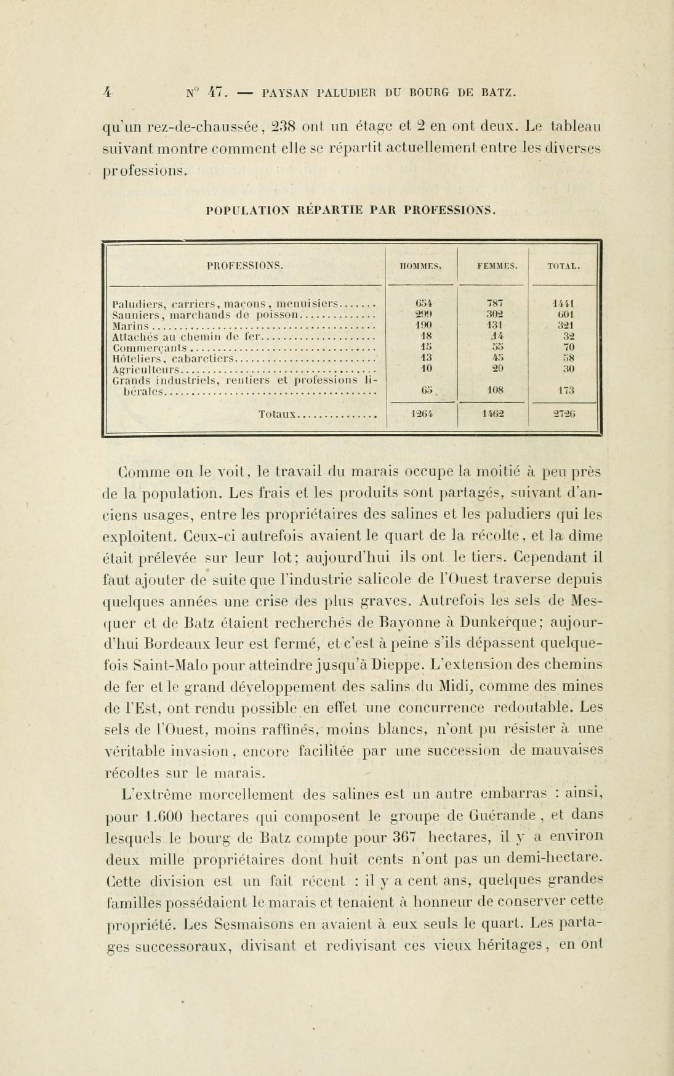
\includegraphics[width=0.8\linewidth]{img/tabl_s2t1_m47_p4.png}
     \caption{s. 2 vol. 1, \no{} 47, p. 4.}
    \end{subfigure}
    \hspace{5pt}
    \begin{subfigure}[t]{0.4\textwidth}
     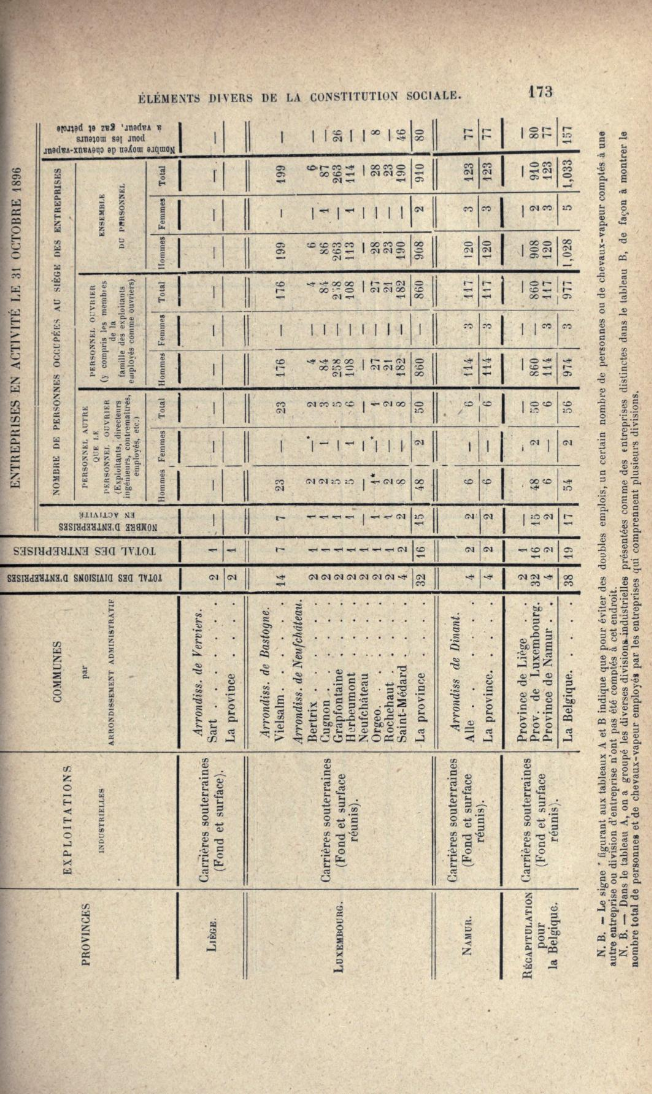
\includegraphics[width=0.8\linewidth]{img/tabl_s3t1_m102_p173.png}
     \caption{s. 3 vol. 1, \no{} 102, p. 173.}
     \label{fig:ex_figures:table}
    \end{subfigure}
    \hspace{5pt}
    
    
    
    \begin{subfigure}[t]{0.4\textwidth}
     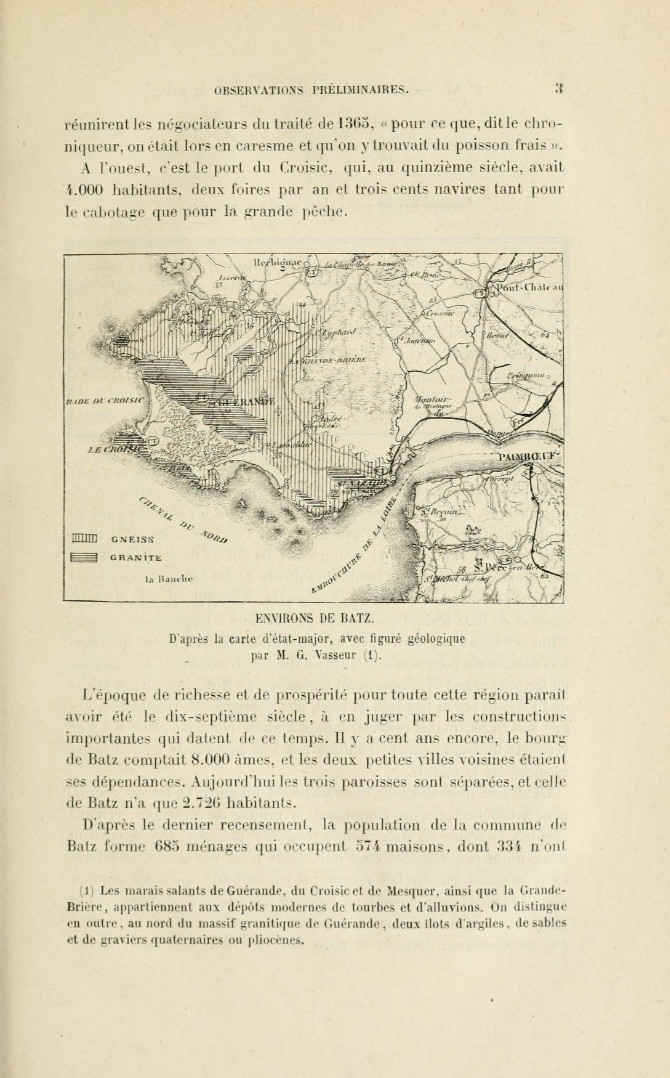
\includegraphics[width=0.8\linewidth]{img/map_s2t1_m47_p3.png}
     \caption{s. 2 vol. 1, \no{} 47, p. 3.}
    \end{subfigure}
    \hspace{5pt}
    \begin{subfigure}[t]{0.4\textwidth}
     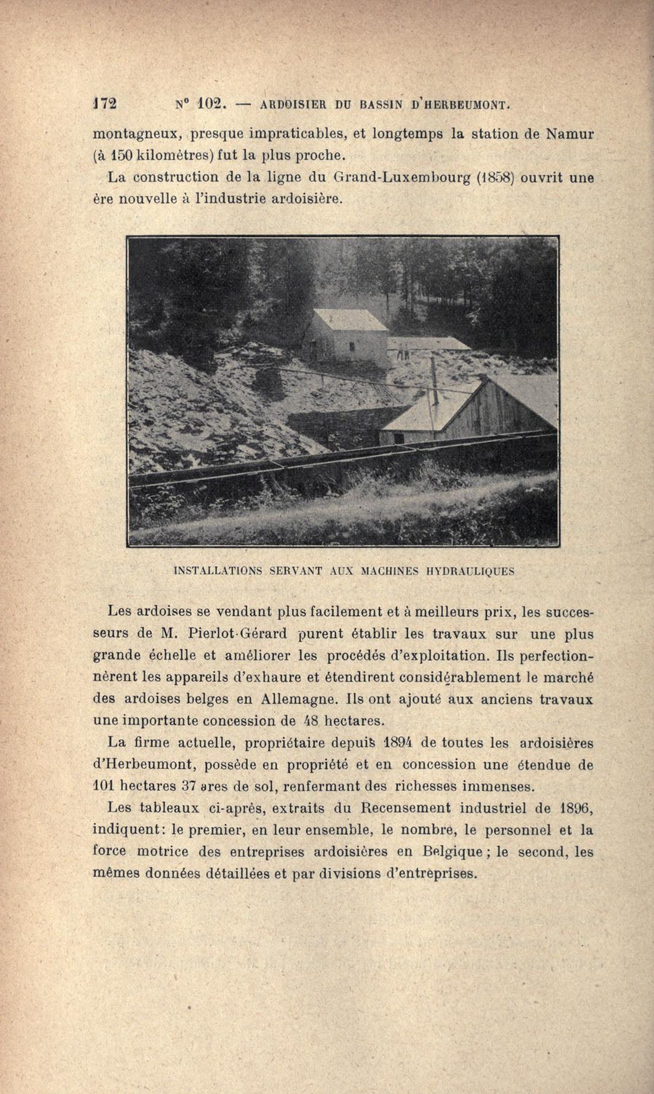
\includegraphics[width=0.8\linewidth]{img/img_s3t1_m102_p172.png}
     \caption{s. 3 vol. 1, \no{} 102, p. 172.}
    \end{subfigure}
    \hspace{5pt}
    \caption[Exemples d'objets graphiques]{Exemples d'objets graphiques dans les pages des \odm{}.}
    \label{fig:ex_figures}
\end{figure}

\lodm{} ne contiennent cependant pas que des chaînes de caractères organisées en lignes. On y trouve des \og objets \fg{} : outre des reproductions de photographies occupant tout ou partie de la page dans les monographies des deuxième et troisième séries, il s'agit principalement de tableaux (\fig{} \ref{fig:ex_figures}). Les paragraphes 14 à 16 consistent ainsi en des tableaux de budget qui s'étendent sur plusieurs pages. Ils suscitent un intérêt particulier pour le programme \timeus{}, dans la mesure où ces budgets permettent de reconstituer les différents postes de dépenses des familles --- et notamment le textile --- et les ressources qui leur sont allouées. Des tableaux peuvent également se trouver dans les autres sections, entre deux paragraphes.

La segmentation en elle-même a été réalisée à l'aide du logiciel \textit{\textsc{abbyy} FineReader}\footnote{\textit{FineReader} produit également une transcription, mais celle-ci est de trop mauvaise qualité pour pouvoir être exploitée}, en tant que service proposé par le logiciel \transkribus{}\footcite{chague2}. Ce dernier est une plate-forme de transcription et d’annotation développée par le programme européen \textsc{read} (\textit{Recognition and Enrichment of Archival Documents})\footnote{Présentation du logiciel : \url{https://readcoop.eu/transkribus/} (consulté le \today).}.

Un total de 6 668 images issues des \odm{} a été chargé dans \transkribus{}. \textit{FineReader} a ensuite analysé leur mise en page et fourni un résultat sous la forme d'un fichier XML ALTO\footcite{alto}. ALTO (\textit{Analyzed Layout and Text Object}) est un format maintenu par la Bibliothèque du Congrès qui \og conserve les informations de mise en page et le texte reconnu par \ocr{} des pages de tout type de documents imprimés \fg\footnote{\og \textit{ALTO stores layout information and OCR recognized text of pages of any kind of printed documents} \fg{} : \og \textit{ALTO Principles} \fg, Bibliothèque du Congrès (\url{https://www.loc.gov/standards/alto/description.html}, consulté le \today).}. Les fichiers ALTO contiennent \og des balises \textit{TextBlock}/\textit{TextLine} renvoyant les coordonnées des lignes de texte, ainsi que des balises \textit{GraphicalElement}, pour les éléments graphiques, qui indiquent notamment les éléments de type \textit{table} \fg\footcite{chague2}.

Il était dès lors possible de passer à la reconnaissance des caractères.

\subsection{Reconnaissance des caractères}

La reconnaissance des caractères est la deuxième étape de l'\ocr. Elle nécessite d'établir un modèle à partir d'une \og vérité terrain \fg{} (\textit{ground truth}), \cad{} la transcription parfaite d'un échantillon du corpus. Le logiciel calcule ensuite le taux de similarité entre les formes qu'il détecte et celles qui se trouvent dans le modèle. Pour ce faire, il détecte le premier caractère de la zone segmentée, identifie ses signes distinctifs et, à partir de ceux-ci, l'associe au symbole du modèle fourni avec qui il partage le plus de points communs\footcite[p.~3]{casey}. Cette séquence est répétée jusqu'à ce que plus aucun caractère ne soit détecté dans le segment, le logiciel réitérant alors l'opération sur le segment suivant jusqu'à arriver au dernier du document.

\begin{figure}[t]
    \centering
    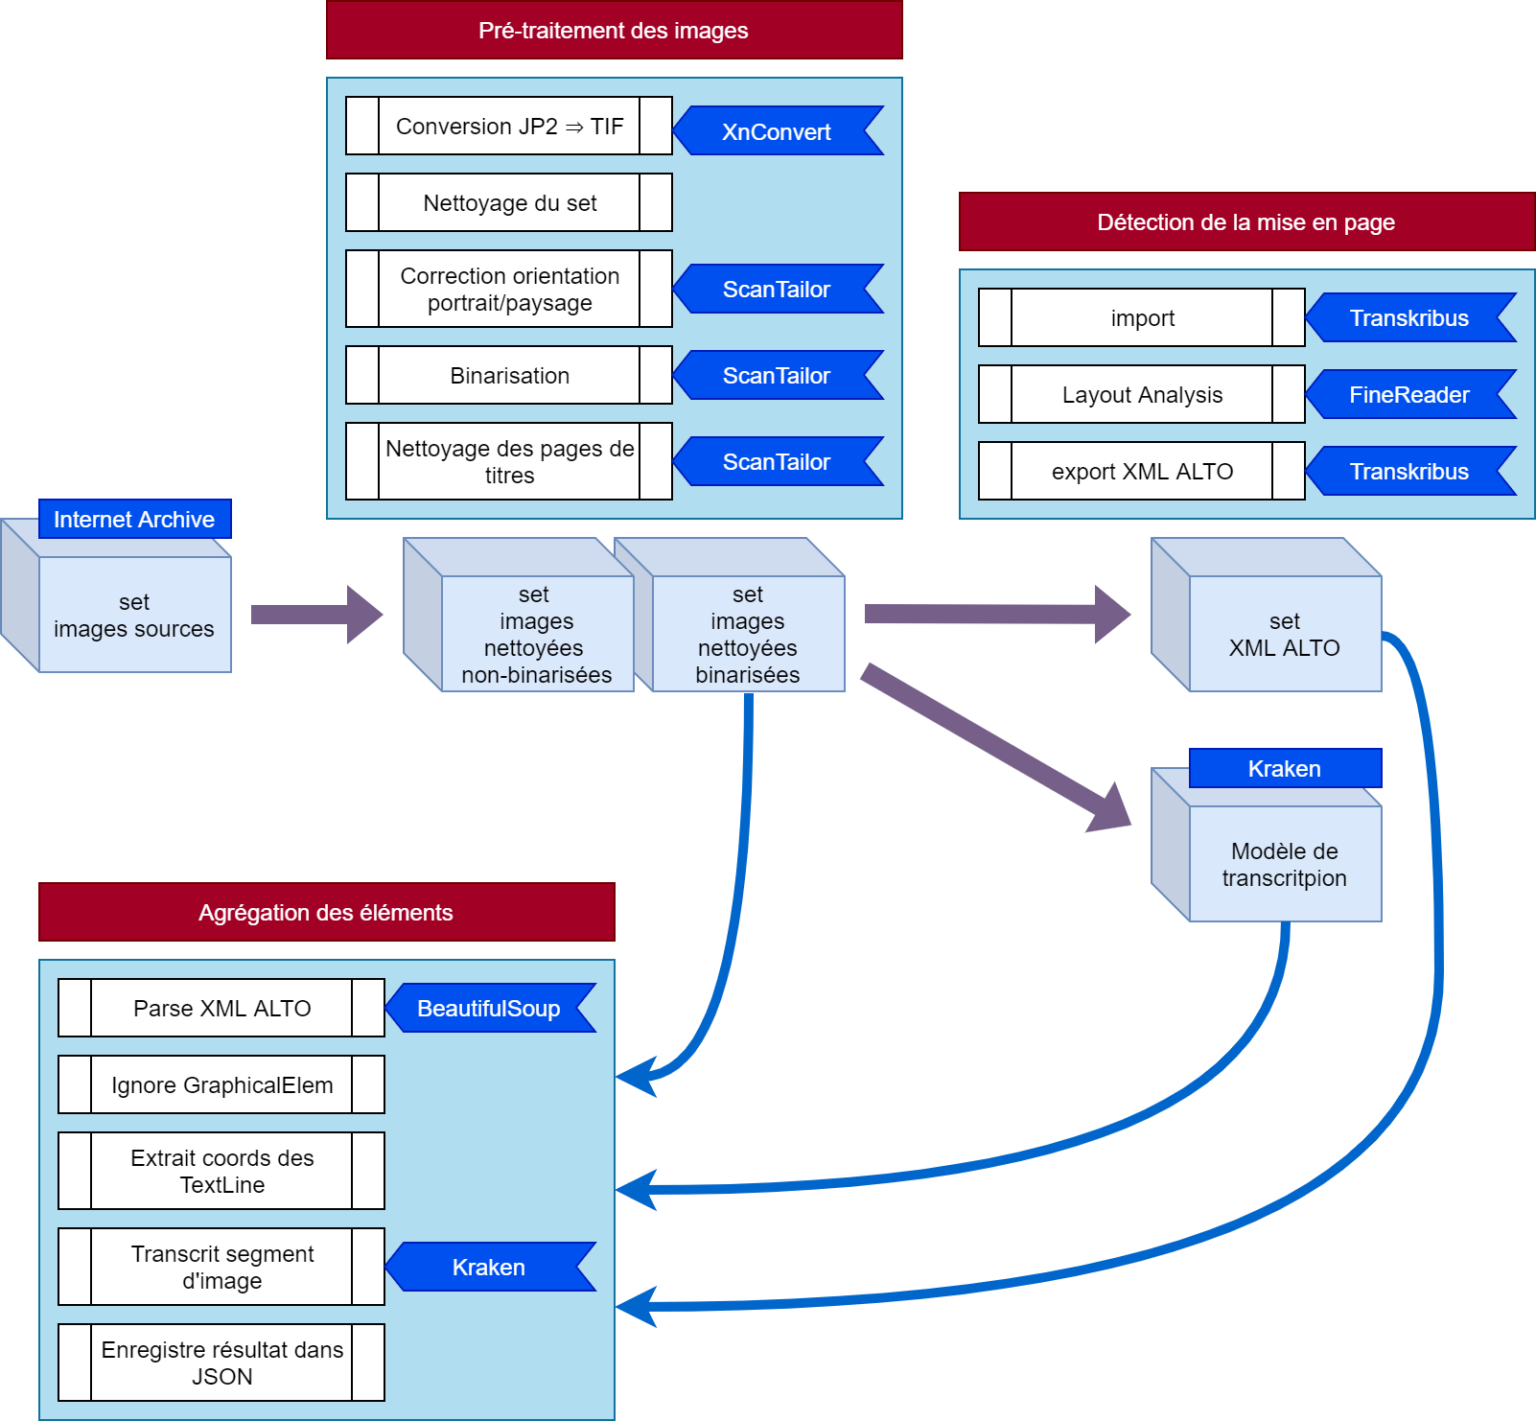
\includegraphics[width=15cm]{img/schema_lse_od2m.png}
    \caption[Schématisation des étapes suivies pour l’extraction du texte et des informations de mise en page]{Schématisation des étapes suivies pour l’extraction du texte et des informations de mise en page (source : Alix Chagué, \url{https://timeus.hypotheses.org/626}).}
    \label{fig:schema_lse_od2m}
\end{figure}

Dans le cadre du projet \timeus, étant donné les choix techniques déjà opérés pour le traitement des autres documents, deux solutions étaient envisageables pour la reconnaissance des caractères des \odm. La première était l'usage de \transkribus{}, la seconde utilisait \kraken{}.

\kraken{} est un logiciel libre développé en Python par Benjamin Kiessling\footnote{Chercheur du laboratoire d'humanités numériques \og Alexander von Humboldt \fg{} de l'Université de Leipzig (\textit{Leipzig  University’s  Alexander  von  Humboldt  Chair for Digital Humanities}). Benjamin Kiessling a également fait partie de l'équipe ALMAnaCH de 2018 à 2019.} à partir du système \textit{OCRopus}\footcite{kiessling}. Dans le processus d'\ocr, \kraken{} se passe de l'étape de la segmentation des mots et des caractères grâce à un \og réseau neuronal artificiel \fg{} qu'il utilise \og pour analyser l'image d'une ligne de texte, la séquence d'entrée, en une suite de caractères, la séquence de sortie \fg{}\footnote{\og \textit{[Kraken's] recognition engine operates as a segmentation-less sequence classifier using an artificial neural network to map an image of a single line of text, the input sequence, into a sequence of characters, the output sequence} : \cite{kiessling}.}. Ce point est l'apport principal de \kraken{} par rapport à tous les logiciels similaires tels que \transkribus{} : grâce à un apprentissage profond (\textit{deep learning}), il peut analyser un nombre important d'écritures de toute époque, latines et même arabes, et en proposer une transcription\footcite{kiesslingarabe}.

\og En 2018 \fg, note cependant Alix Chagué, \og il n’était pas possible d’obtenir une analyse de la mise en page complète avec \kraken \fg{}\footcite{chague2}. Mais le logiciel permettait déjà d'entraîner un modèle pour l'\ocr. Cela était également possible avec \transkribus, mais le fichier modèle ne peut pas être exporté depuis cette plate-forme, alors que l'opération est possible avec \kraken{}, qui donne de meilleurs résultats, sous la forme de fichiers \texttt{.mlmodel}. L'équipe ALMAnaCH a donc choisi de recourir à \kraken{} pour la phase de transcription (entraînement du modèle puis reconnaissance des caractères)\footcite{chague2}.

Les fichiers \og vérité terrain \fg{} étaient composés des transcriptions de 1300 lignes (fichiers texte) et de leurs images (fichiers image). Pour s'entraîner, \kraken{} itère sur chaque couple de fichiers, transcrit le fichier image et compare le résultat au contenu du fichier texte. Le passage en revue de l'ensemble des données (ici, les 1300 paires) constitue une \textit{epoch}. Un taux de réussite (\textit{accuracy report}) est calculé à la fin de chaque itération. Il se compose de trois données numériques : le taux de réussite (positif ou négatif), le nombre de caractères contenus dans l'\textit{epoch} et les faux-positifs (\cad{} le nombre de caractères mal reconnus). Plusieurs dizaines d'\textit{epochs} sont nécessaires pour parvenir à un taux de réussite optimal et donc à un modèle fiable (\fig{} \ref{fig:kraken_training}).

\begin{figure}
    \centering
    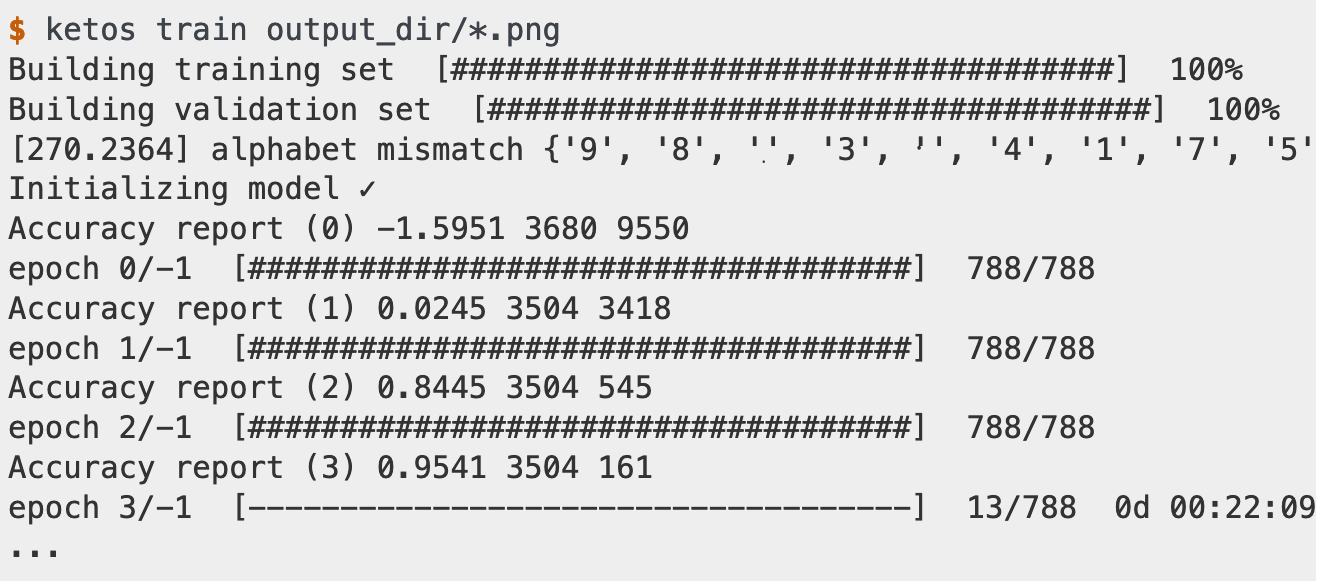
\includegraphics[width=15cm]{img/kraken_training.png}
    \caption[Exemple d'un entraînement opéré par \kraken]{Exemple d'un entraînement opéré par \kraken. Trois \textit{epochs} (\no{} 0 à 2) sont arrivées à leur terme, la quatrième étant en cours de chargement (\no{} 3). Le taux de réussite augmente à chaque nouvelle \textit{epoch} : de \texttt{-1.5951} pour la première (\texttt{9550} fautes sur... \texttt{3680} caractères détectés), il atteint \texttt{0.8445} pour la troisième (\texttt{545} fautes sur \texttt{3504} caractères détectés). Capture d'écran du site de \kraken{} (\url{http://kraken.re/training.html}, consulté le \today).}
    \label{fig:kraken_training}
\end{figure}

Une fois ce modèle obtenu, la phase de transcription automatique pouvait commencer. \kraken{} pouvant être utilisé comme une librairie du langage Python, il a pu être envisagé de fédérer les étapes de transcription et d'encodage des textes obtenus sous l'égide d'un même script, \lse. Son fonctionnement débute ainsi :

\begin{enumerate}
    \item Il prend pour paramètres les fichiers images des \odm{} et les fichiers ALTO produit par \transkribus ;
    \item Chaque image est associé à son fichier ALTO ;
    \item Les coordonnées des lignes de texte sont extraits de l'ALTO et le script lance la transcription de ces lignes à l'aide de \kraken{} et du modèle précédemment obtenu.
    \item Les transcriptions de chacune des 6 608 images sont stockées dans autant de fichiers XML-TEI.
\end{enumerate}

Ces transcriptions relèvent du texte brut, \cad{} que la donnée n'y est pas structurée.

\subsection{Structuration}

C'est à ce stade que l'analyse de la structure logique menée précédemment est prise en compte (\ann{} \ref{structure}).

\begin{enumerate}
    \item Les limites des chapitres (monographies et éléments de paratexte) sont identifiées en fonction des pages de titres qui marquent le début de celui en cours et la fin du précédent.
    \item Les transcriptions sont rassemblées par chapitre.
    \item Si un chapitre est identifié comme étant une monographie, alors le script y lance une recherche pour détecter les titres de la structure logique. Le script est rendu tolérant par une distance de Levenshtein (ou distance d'édition) souple afin de reconnaître un titre en dépit d'une transcription partiellement fautive. La distance de Levenshtein mesure l'écart entre deux chaînes de caractères, ici entre le modèle (le titre standard) et sa transcription.
    \item Un arbre XML est créé en respectant les différents niveaux de la structure logique.
    \item En sortie, le script renvoie :
    \begin{itemize}
        \item Treize fichiers \og source \fg{} avec le contenu de chaque volume ;
        \item Deux cent vingt-trois fichiers correspondant à autant de chapitres détectés.
    \end{itemize}
\end{enumerate}

\section{Les fichiers XML-TEI}

Ces fichiers XML sont structurés avec un schéma TEI.

XML (\textit{Extensible Markup Language}, en français \textit{langage de balisage extensible}) est un format de données conçu pour la description des documents textuels, ne possédant pas de jeu de balises prédéfini\footnote{Définition d'Ariane Pinche : \url{https://github.com/ArianePinche/coursTNAH_XML-TEI/blob/master/seance01/InitiationXML.md} (consulté le \today).}.

La TEI (\textit{Text Encoding Initiative}) est un schéma de données XML commencé en 1987 dont le but est de \og fournir des recommandations pour la création et la gestion sous forme numérique de tout type de données créées et utilisées par les chercheurs en sciences humaines \fg\footcite[p. 9]{burnard}. Ses trois caractéristiques principales sont qu'il \og s’intéresse au sens du texte plutôt qu'à son apparence \fg, qu'il est \og indépendant de tout environnement logiciel particulier \fg{} et qu'il a été conçu par une communauté scientifique qui le maintient toujours aujourd'hui à travers le \textit{TEI Consortium} fondé en 2000\footcite[p. 9]{burnard}. 

Ce format conjugue ainsi une certaine \og flexibilité et un intérêt centré sur les besoins scientifiques \fg\footcite[p. 10]{burnard}. L'utiliser pour encoder les transcriptions des \odm, c'est donc décrire de la meilleure manière possible l'organisation originale du texte dans les volumes imprimés tout en assurant la pérennité de la donnée ainsi produite.

Un document XML peut être représenté sous une forme arborescente, \og l'arbre XML \fg{} (\fig{} \ref{fig:xmltree1}). Il débute par un élément racine (\texttt{<TEI>}) qui contient tous les autres.

Les trois grandes sections de l'arbre sont le \texttt{<teiHeaer>}, les \texttt{<facsimile>} et le \texttt{<text>}. Le \texttt{<teiHeaer>} est l'en-tête où se trouvent les métadonnées du document. Il est ici réduit à son minimum, n'étant composé que d'une description bibliographique (\texttt{<fileDesc>}) : le titre et ses auteurs (\texttt{<titleStmt>}), l'organisation responsable de la publication, la date et le lieu de celle-ci (\texttt{<publicationStmt>}), et enfin une description sommaire des \odm{} (\texttt{<sourceDesc>})\footnote{\og Les \odm{} sont des recueils d'enquêtes sociologiques publiées pendant la deuxième moitié du \textsc{xix}\ieme{} siècle. Ces enquêtes ont été rassemblées sous la forme de 3 séries de plusieurs volumes. Accès aux fichiers images sources : \url{http://timeusage.paris.inria.fr/mediawiki/index.php/Aperçu_des_états\#Les_Ouvriers_des_Mondes} \fg.}. L'en-tête contient également un \texttt{<encodingDesc>} où le lien est fait avec le programme ANR ; l'action du script \lse{} est également mentionnée\footnote{\og Cette édition numérique des \odm{} a été réalisée dans le cadre du projet ANR \timeus{} (\url{http://larhra.ish-lyon.cnrs.fr/anr-time-us}). Elle est générée automatiquement grâce au programme \lse{} (\url{https://gitlab.inria.fr/almanach/time-us/LSE-OD2M}), développé par Alix Chagué, équipe Inria ALAMAnaCH \fg.}.

\begin{figure}
    \centering
    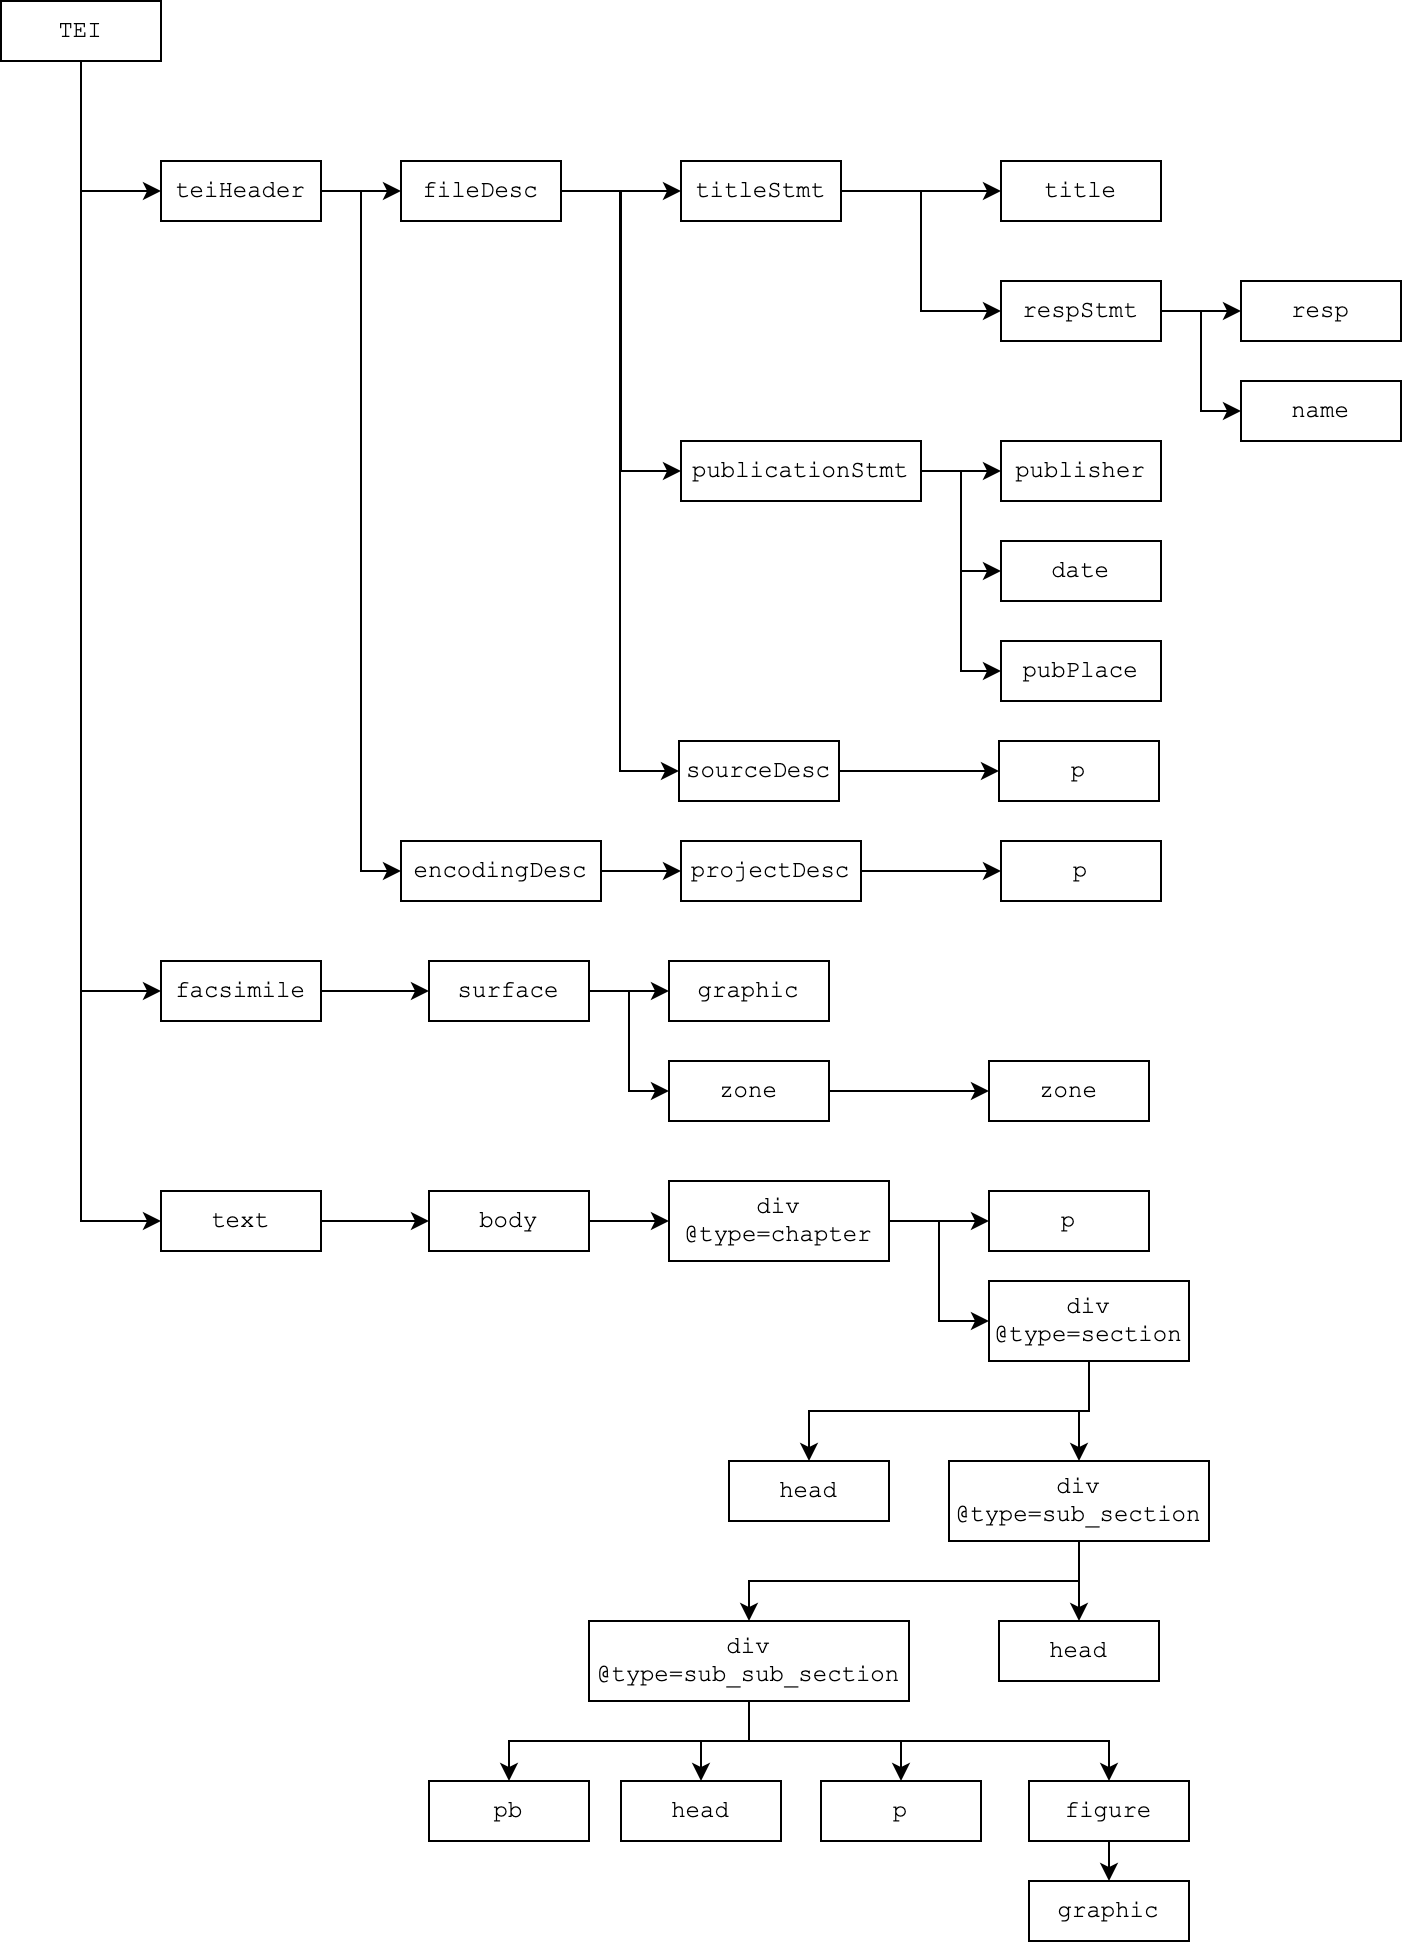
\includegraphics[width=16cm]{img/xml_tree_1.png}
    \caption[Représentation de l'arbre XML des fichiers TEI]{Représentation de l'arbre XML utilisé par le script \lse{} pour encoder les transcriptions des monographies des \odm.}
    \label{fig:xmltree1}
\end{figure}

Le document continue avec une succession de balises \texttt{<facsimile>} dont le but est de conserver le lien entre le texte et son segment dans l'image d'origine (\fig{} \ref{fig:facsimile})\footnote{\textit{TEI Guidelines, 11 Representation of Primary Sources, 11.1 Digital Facsimiles} (\url{https://tei-c.org/release/doc/tei-p5-doc/fr/html/PH.html\#PHFAX}, consulté le \today).}. L'élément suivant, \texttt{<surface>}, possède quatre attributs : \texttt{@ulx} et \texttt{@uly} qui ont pour valeurs l'abscisse \textit{x} et l'ordonnée \textit{y} du coin supérieur gauche du bloc de segmentation (la page), et \texttt{@urx} et \texttt{@ury} contenant les valeurs de l'abscisse \textit{x} et de l'ordonnée \textit{y} du coin inférieur droit. Ces coordonnées sont directement reprises des fichiers XML ALTO obtenus avec \textit{FineReader}. On trouve ensuite un élément \texttt{<graphic>} avec un attribut \texttt{@url} ayant pour valeur le chemin local vers l'image de la page, et un élément \texttt{<zone>} contenant lui-même un ensemble de balises \texttt{<zone>}. Ces dernières contiennent les coordonnées des blocs de segmentation à l'intérieur du bloc supérieur définit par \texttt{<surface>} ; ces sous-blocs sont catégorisés par un attribut \texttt{@rendition} ayant pour valeur \texttt{paragraph} lorsqu'il s'agit de texte ou \texttt{table} pour un tableau.

\begin{figure}
    \centering
    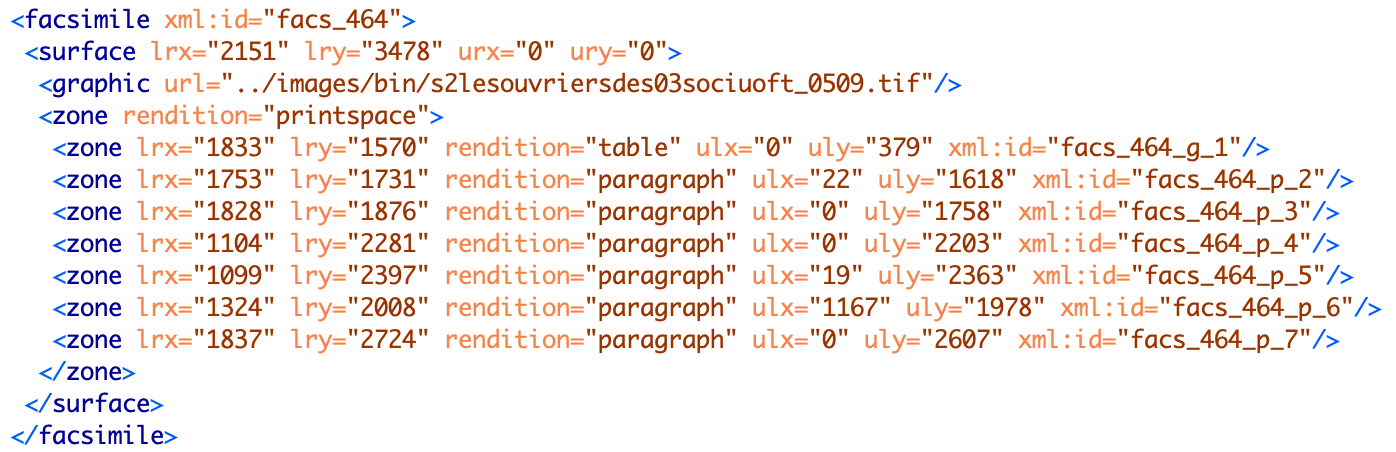
\includegraphics[width=16cm]{img/facsimile.png}
    \caption[Exemple d'un ensemble \texttt{<facsimile>}]{Exemple d'un ensemble \texttt{<facsimile>} dans le fichier source du troisième volume de la deuxième série.}
    \label{fig:facsimile}
\end{figure}

Le \texttt{<teiHeaer>} et les éléments \texttt{<facsimile>} montrent que la structuration d'un texte brut issu d'une \ocr{} ne consiste pas simplement en l'encodage de la transcription. Il s'agit aussi de produire des métadonnées permettant de décrire le contenu du fichier.

La dernière section de l'arbre, \texttt{<text>}, contient les transcriptions structurées au sein de son élément \texttt{<body>}. Notons que l'implémentation de la structure logique par \lse{} n'a pas donné de résultats optimaux et a fait l'objet d'une reprise majeure lors du stage. Ces résultats restent néanmoins satisfaisants au regard du temps alloué pour l'écriture et le fonctionnement du  script (trois mois). 

Le principe retenu est le suivant : chaque division de la structure est enchâssée dans un élément \texttt{<div>} pour lequel un attribut \texttt{@type} vient préciser son niveau. De manière assez classique, cet encodage traduit ainsi la hiérarchie sémantique interne aux monographie grâce à une imbrication de \texttt{<div>} jusqu'à arriver au texte lui-même\footcite[p. 117]{clerice}. Les valeurs de l'attribut \texttt{@type} sont calquées sur les divisions des documents du langage de composition \LaTeX{} : \texttt{\textbackslash chapter\{\}}, \texttt{\textbackslash section\{\}}, \texttt{\textbackslash subsection\{\}}, \texttt{\textbackslash subsubsection\{\}}. Cela a pour but de faciliter une éventuelle transformation des documents XML-TEI au format \LaTeX\footcite[p. 52]{chague2}.

La monographie correspond à une \texttt{<div>} de type \texttt{chapter}. Les ensembles de niveau~A (page de titre, \textit{Observations préliminaires} et \textit{Notes}) sont de type \texttt{section}, les titres de niveau~I \texttt{sub\_section} et les paragraphes \texttt{sub\_sub\_section} (\textit{cf.} \ann{} \ref{structure}). Dans chaque niveau, le titre en lui-même est encodé au sein d'un élément \texttt{<head>}, le texte se trouvant ensuite dans des \texttt{<p>} (\fig{} \ref{fig:ex_structure}).

Pour les éléments de paratexte, tels que les avertissements liminaires de chaque volume, seul le niveau \texttt{chapter} a été utilisé, l'ensemble du texte se trouvant dans des \texttt{<p>}.

\begin{figure}[t]
    \centering
    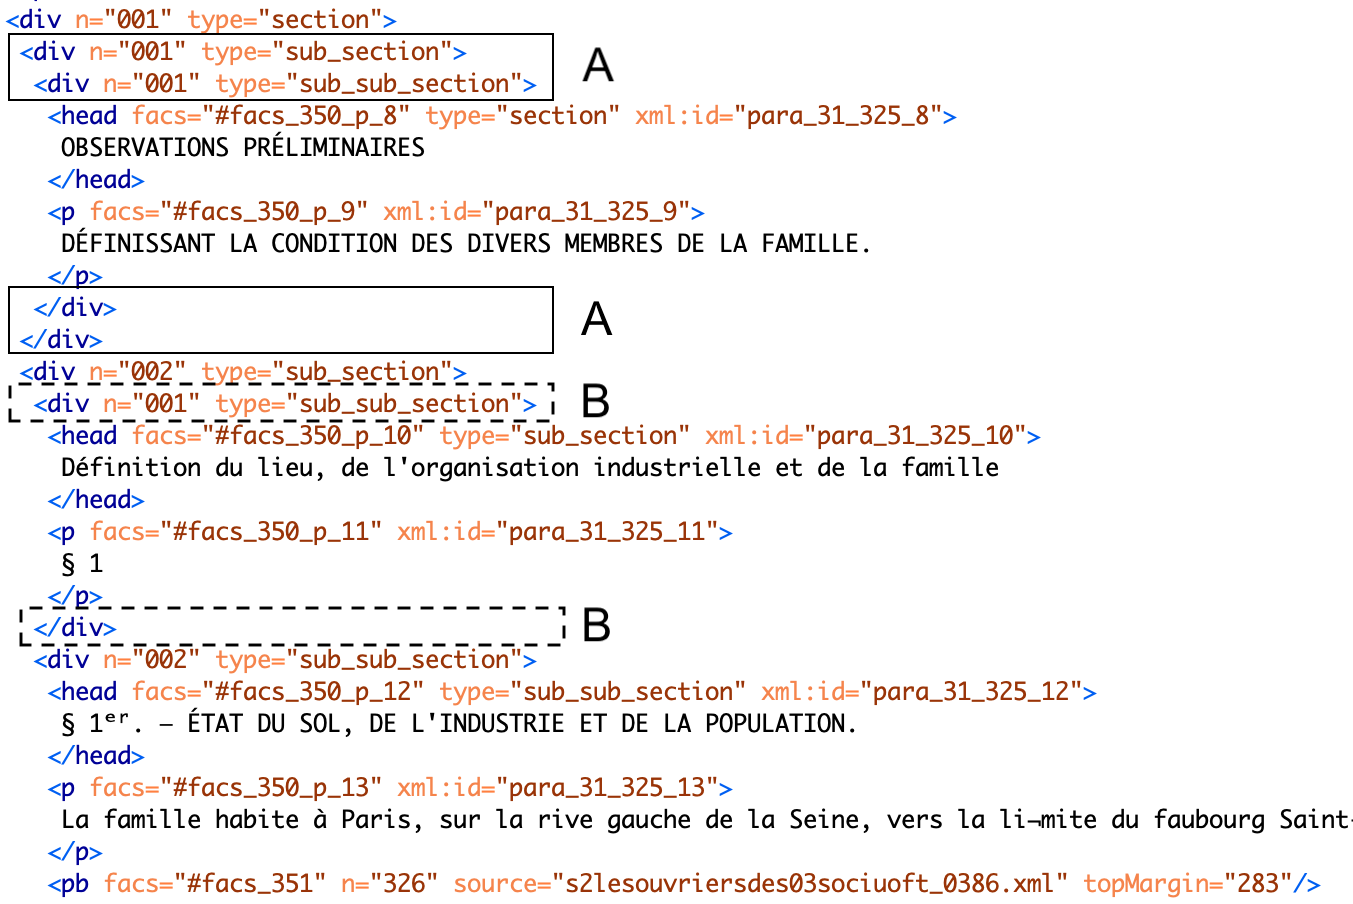
\includegraphics[width=16cm]{img/ex_structure.png}
    \caption[Exemple de la structuration du début de la monographie \no{} 70]{Exemple de la structuration du début des \textit{Observations préliminaires} de la monographie \no{} 70 par le script \lse{} (\texttt{s2t3\_chapt\_31.xml}). L'encodage est fautif dans la mesure où des niveaux supplémentaires ont été rajoutés : \textit{Observations...} ne devrait être que dans une \texttt{section} (les lignes des repères A n'ont pas lieu d'être), \textit{Définitions du lieu...} dans une \texttt{sub\_section} (les lignes des repères B sont fautives). On remarque également une erreur de transcription, le numéro de paragraphe (§1) étant répété. La balise finale, \texttt{<pb>}, marque un changement de page.}
    \label{fig:ex_structure}
\end{figure}

Le script \lse{} a été lancé sur le \textit{cluster} (ou \textit{grappe de serveurs}) \rioc{} d'Inria, où il a fallu un peu plus de quinze heures pour traiter l'ensemble des \odm. Un \textit{cluster} est un groupe d'ordinateurs inter-connectés où une \og reine \fg{} (le \textit{master node}) répartit grâce à un \og planificateur \fg{} (\textit{scheduler}) les tâches qui lui sont demandées à des \og ouvrières \fg{} (les \textit{slave nodes})\footnote{\textit{\rioc{} Architecture}, \url{https://sed-paris.gitlabpages.inria.fr/rioc/rioc_architecture/rioc_architecture.html} (consulté le \today).}. Quatre des \og ouvrières \fg{} de \rioc{} possèdent des GPU (\textit{graphics processing unit}). Équipées d'une carte graphique, ces processeurs sont capables de réaliser du calcul vectoriel et peuvent ainsi traiter les images --- par exemple les pages des \odm{} --- très rapidement. Cette architecture en réseau permet d'augmenter de façon significative la vitesse de calcul et donc l'exécution des tâches.

Au final, les treize fichiers source créés par \lse{} représentent 25,5 Mo. Ils ont été divisés en 223 fichiers (25,7 Mo) nommés de la façon suivante : \texttt{s[numéro de la série]t[numéro du volume]\_chapt\_[numéro du chapitre dans le volume].xml} (\ann{} \ref{mapping}).

\clearpage

\vspace*{\stretch{0.3}}

Au moment de commencer notre stage, nous avons donc trouvé un ensemble de 223 fichiers XML contenant les transcriptions structurées avec un schéma TEI des treize volumes des \odm. Les fichiers contenaient des enquêtes sociologiques (les monographies) et des éléments de paratexte. Les chercheurs et les chercheuses du programme ANR \timeus{} n'étaient intéressés que par les monographies, mais Inria avait la volonté de valoriser l'ensemble des fichiers.

Plusieurs points avaient été identifiés comme posant problème pour une future valorisation sous la forme d'une publication ou d'une réutilisation dans des projets de traitement automatique du langage (TAL).

Nous allons à présent exposer les différentes reprises que nous avons menées.
\vspace*{\stretch{1.7}}